\section{Prism}
\label{sec:Prism}

\begin{figure}[!ht]
\begin{center}
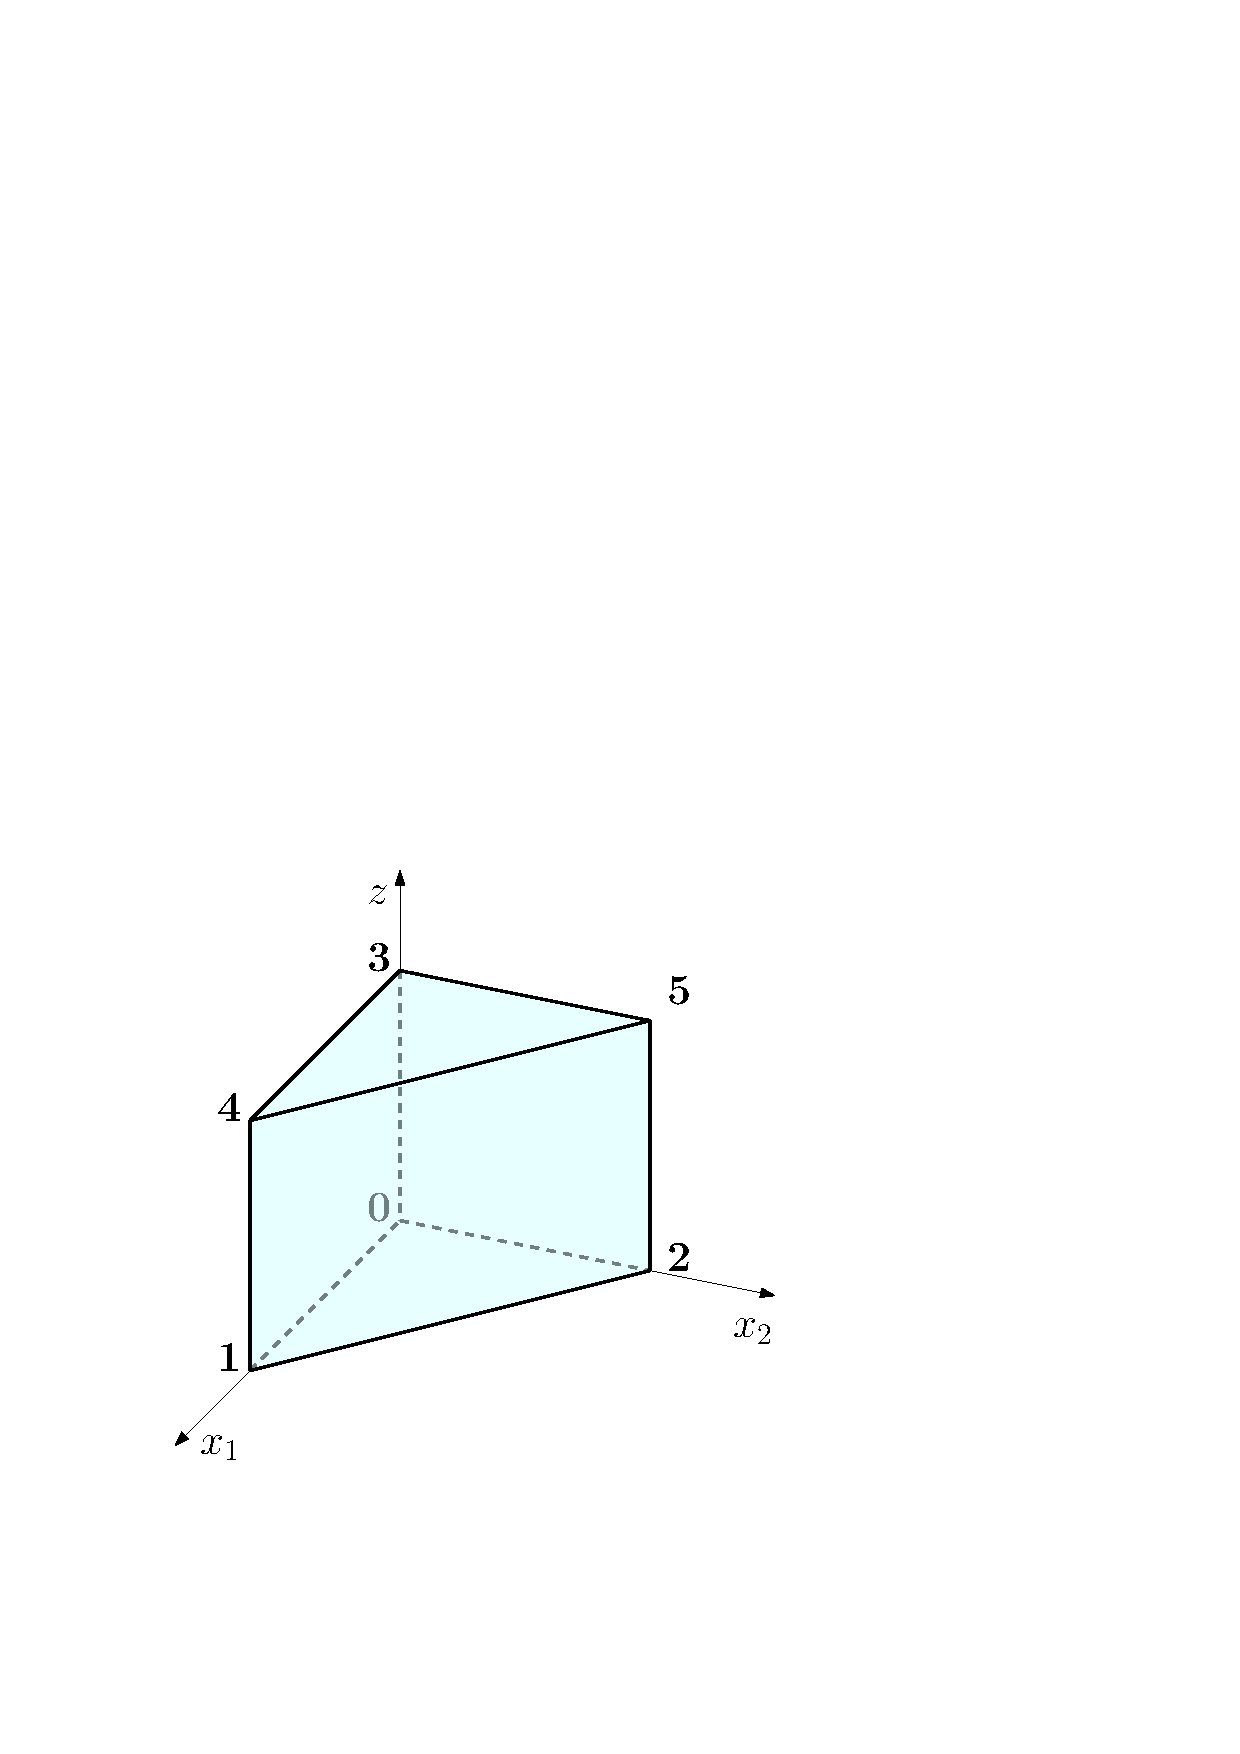
\includegraphics[scale=0.5]{./figures/MasterPrism.pdf}
\caption{Master prism with numbered vertices.}
\label{fig:MasterPrism}
\end{center}
\end{figure}

The master prism is shown in Figure \ref{fig:MasterPrism} in the $(x,z)=(x_1,x_2,z)$ space.
It is the Cartesian product of a triangle and a segment.
More specifically, it is $\{x\in\R^2:x_1>0,x_2>0,x_1+x_2<1\}\times(0,1)$.
Here, $x$ represents the triangle element coordinates, while $z$ represents the 1D segment element coordinate.

%The prism element can be viewed as the Cartesian product of the 2D triangle element and the 1D segment element. 
%The master element is shown in Figure \textit{addFig} in the $(x,z)$ space, where $x=(x_1,x_2)$. 
%Here, $x$ represents the triangle element coordinates, while $z$ represents the 1D segment element coordinate.

The prism has both quadrilateral and triangle faces. 
Similarly, there are two types of edges. 
Those edges which are adjacent to both a quadrilateral face and a triangle face are called \textit{mixed edges}, while those edges only shared by quadrilateral faces are simply called \textit{quadrilateral edges}. 
These distinctions are important, and the form of the shape functions will differ for the different types of edges and faces.

Due to the Cartesian product structure, it is natural to consider the 2D affine coordinates for the triangle (dependent on $x$) and the 1D affine coordinates for the segment (dependent on $z$). 
For this master element they are
\begin{equation}
	\begin{gathered}
		\nu_0(x)=1-x_1-x_2\,,\qquad\nu_1(x)=x_1\,,\qquad\nu_2(x)=x_2\,,\\
		\mu_0(z)=1-z\,,\qquad\quad\mu_1(z)=z\,.
	\end{gathered}
\end{equation}
Their gradients in 3D are
\begin{equation}
	\begin{gathered}
		\nabla\nu_0(x)=\bigg(\begin{smallmatrix}-1\\[2pt]-1\\[2pt]0\end{smallmatrix}\bigg)\,,\qquad
			\nabla\nu_1(x)=\bigg(\begin{smallmatrix}1\\[2pt]0\\[2pt]0\end{smallmatrix}\bigg)\,,\qquad
				\nabla\nu_2(x)=\bigg(\begin{smallmatrix}0\\[2pt]1\\[2pt]0\end{smallmatrix}\bigg)\,,\\
		\nabla\mu_0(z)=\bigg(\begin{smallmatrix}0\\[2pt]0\\[2pt]-1\end{smallmatrix}\bigg)\,,\qquad\quad
			\nabla\mu_1(z)=\bigg(\begin{smallmatrix}0\\[2pt]0\\[2pt]1\end{smallmatrix}\bigg)\,.
	\end{gathered}
\end{equation}
These are important and are used explicitly or implicitly in many of the oncoming calculations.

As usual, there are natural relationships between vertices, edges and faces, and the affine coordinates.
The related coordinates are those which take the value $1$ at the given topological entity.
In fact, for the prism each vertex is linked to \textit{two} affine coordinates, one of them a 2D affine coordinate and the other a 1D affine coordinate.
Moreover, each edge is linked to \textit{one} affine coordinate.
For mixed edges it is a 1D affine coordinate, while for quadrilateral edges it is a 2D affine coordinate.
Lastly, the triangle faces are also linked to \textit{one} 1D affine coordinate.
For example, vertex $0$, $v_0=(0,0,0)$, is linked to the affine coordinates $\nu_0(x)$ and $\mu_0(z)$.
Meanwhile, mixed edge 01 is linked to the affine coordinate $\mu_0(z)$, while quadrilateral edge 03 is linked to the affine coordinate $\nu_0(x)$.
Finally, face 012 is linked to $\mu_0(z)$.

\subsubsection*{Exact Sequence}

%Recall the 3D exact sequence
%\begin{equation*}
%H^1\,\xrightarrow{\nabla}\,H(\text{curl})\,\xrightarrow{\nabla\times}\,H(\text{div})\,\xrightarrow{\nabla\cdot}\,L^2\,.
%\end{equation*}
%
%As suggested by the structure of the prism, one would naturally expect the shape functions to be products or some combination of the corresponding shape functions of the triangle and segment element. 
%Indeed, this is the case. 
The product structure of the prism suggests that the discrete polynomial exact sequence approximating \eqref{eq:3D_exact_sequence} is intimately related to the discrete sequences for the triangle and segment (see \eqref{eq:EStriangle} and \eqref{eq:ESsegment}).
Indeed, this is the case. 
The sequence is of the form
%It is reflected as well in the discrete polynomial spaces in the exact sequence of the element, which are intricately related to the exact sequences for the triangle and line segment respectively (see \eqref{eq:EStriangle} and \eqref{eq:ESsegment}).
%Let $\mathcal{P}^p =\mathcal{P}^p(x_1,x_2)$ be the space of polynomials of total order $p$ in the $x=(x_1,x_2)$ space, and $\mathcal{P}^q=\mathcal{P}^q(z)$ be the space of polynomials of order $q$ in the $z$ variable. 
%Similarly, recall the definitions of the spaces $\mathcal{N}^p$ and $\mathcal{RT}^p$ in $N=2$ spatial dimensions given in \eqref{eq:NedelecSpace} and \eqref{eq:RaviartThomasSpace} which are assumed to be in the $x=(x_1,x_2)$ space. 
%Then, the finite dimensional exact sequence is of the form 
\begin{equation}
	W^{p,q} \xrightarrow{\,\,\nabla\,\,} Q^{p,q} \xrightarrow{\nabla\times} V^{p,q} \xrightarrow{\nabla\cdot} Y^{p,q} \,,
\end{equation}
where
\begin{equation}
	\begin{aligned}
	W^{p,q}&=\mathcal{P}^p\otimes\mathcal{P}^q=\mathcal{P}^p(x_1,x_2)\otimes\mathcal{P}^q(z)\,,\\
	Q^{p,q}&=(\mathcal{N}^p\otimes\mathcal{P}^q)\times(\mathcal{P}^p\otimes\mathcal{P}^{q-1})\,,\\
	V^{p,q}&=(\mathcal{RT}^p\otimes\mathcal{P}^{q-1})\times(\mathcal{P}^{p-1}\otimes\mathcal{P}^q)\,,\\
	Y^{p,q}&=\mathcal{P}^{p-1}\otimes\mathcal{P}^{q-1}\,.
	\end{aligned}
\end{equation}
Here, the spaces $\mathcal{N}^p$ and $\mathcal{RT}^p$ correspond to the $N=2$ case (see \eqref{eq:NedelecSpace} and	\eqref{eq:RaviartThomasSpace}), so that the space $\mathcal{N}^p\otimes\mathcal{P}^q=\{\phi E:\phi\in\mathcal{P}^q,E\in\mathcal{N}^p\}$ has two components and dimension $p(p+2)(q+1)$. The same applies to $\mathcal{RT}^p\otimes\mathcal{P}^{q-1}$ which has dimension $p(p+2)q$.


% will be an extension of the corresponding analysis of the triangle and line segment elements. 
%We will denote by $\hat{\Tri}$ the master triangle element, by $\hat{\mathrm{E}} $ the master line segment element, and by $\hat{\Lambda}$ the master prismatic element given as: \begin{equation} \hat{\Lambda} = \hat{\Tri} \times \hat{\mathrm{E}}\end{equation}

%Recall that the affine coordinate functions for the segment are denoted by $\mu_0, \mu_1$ \begin{equation}\mu_1(z)=z, \mu_0(z)=1-z, \mu_0+\mu_1=1 \end{equation} and for the triangle are denoted by \begin{equation}\nu_0(x,y)=1-x-y,\,\nu_1(x,y)=x,\,\nu_2(x,y)=y, \text{ with }\nu_0(x,y)+\nu_1(x,y)+\nu_2(x,y)=1.\end{equation}We will be needing the gradients (in 3D) of the above functions, which we record here: \begin{equation}\nabla \mu_1(z)=(0,0,1)^T,\text{ } \nabla \mu_0(z)= (0,0,-1)^T \end{equation}and \begin{equation}\nabla \nu_0(x,y) = \left(
%\begin{array}{c}
%-1\\
%-1\\
%0 \\
%\end{array}
%\right),\\ \nabla \nu_1(x,y) = \left(
%\begin{array}{c}
%1\\
%0\\
%0 \\
%\end{array}
%\right),\\
%\nabla \nu_2(x,y) = \left(
%\begin{array}{c}
%0\\
%1\\
%0\\
%\end{array}
%\right). \end{equation}
%The prism consists of two triangle faces, of which the ``top" face corresponds to $z=1$ and the ``bottom" face corresponds to $z=0$. We shall henceforth denote the arguments of all shape functions defined on the triangle element as $(x,y)$ and the argument of shape functions defined on the segment will be $z$, so that, for example, the affine function $\nu_0$ defined on the triangle will be written as $\nu_0(x,y)$ while the affine function defined $\mu_0$ on the interval as $\mu_0(z)$. This seperation of variables will allow us to see the tensor product structure more clearly.

%\subsubsection*{Exact Sequences for the Prismatic Element}
%Recall the exact sequence for the triangle element given by the N\'{e}d\'{e}lec/Raviart-Thomas characterization:
%\begin{equation}
%\begin{array}{ccccc} 
%\mathcal{P}^p(\hat{\Tri}) & \stackrel{\nabla}{\longrightarrow} & \mathcal{N}^p & \stackrel{\text{curl(}\cdot{)}}{\longrightarrow}\mathcal{P}^{p-1}(\hat{\Tri})\\ 
%\end{array},\end{equation}
%and,
%\begin{equation}
%\begin{array}{ccccc} 
%\mathcal{P}^p(\hat{\Tri}) & \stackrel{\nabla \times}{\longrightarrow} & \mathcal{R}\mathcal{T}^p & \stackrel{\nabla \cdot}{\longrightarrow}\mathcal{P}^{p-1}(\hat{\Tri})\\ 
%\end{array},\end{equation}
%where the spaces $\mathcal{N}^p$ and $\mathcal{R}\mathcal{T}^p$ are characterized by \begin{equation}\mathcal{N}^p := (\mathcal{P}^{p-1})^{2}\oplus\{ E\in (\tilde{\mathcal{P}^p})^{2}:{x}\cdot E(x)=0 \text{ } \forall x\}\end{equation}
%and \begin{equation}\mathcal{R}\mathcal{T}^p = (\mathcal{P}^{p-1})^{2}\oplus\{ {x}\phi({x}): \phi \in \tilde{\mathcal{P}}^{p-1}\}\end{equation} and are the N\'{e}d\'{e}lec and Raviart-Thomas spaces respectively. Following the presentation in , we have the following exact sequence for the prismatic element: 
%\begin{equation}\begin{array}{ccccc} 
%{W}^{p,q} & \stackrel{\nabla}{\longrightarrow} & {{Q}}^{p,q} & \stackrel{\nabla\times}{\longrightarrow}{V}^{p,q} & \stackrel{\nabla\cdot}{\longrightarrow}{Y}^{p,q}\\ 
%\end{array}, \end{equation}
%where we have:
%\begin{eqnarray}
% {W}^{p,q} &=& \mathcal{P}^p\otimes\mathcal{P}^q      \nonumber \\
% {Q}^{p,q} &=& (\mathcal{N}^p\otimes(\mathcal{P}^q\times\mathcal{P}^q))\times(\mathcal{P}^p\otimes\mathcal{P}^{q-1}) \nonumber \\
%  {V}^{p,q} &=& (\mathcal{RT}^p\otimes(\mathcal{P}^{q-1}\times\mathcal{P}^{q-1}))\times(\mathcal{P}^{p-1}\otimes\mathcal{P}^q) \nonumber \\
%  {Y}^{p,q} &=& \mathcal{P}^{p-1}\otimes\mathcal{P}^{q-1}.
%\end{eqnarray}
%We now discuss the shape functions for the prismatic element.

\subsection{\texorpdfstring{$H^1$}{H1} Shape Functions}
It will be clear that all shape functions lie in $\mathcal{P}^p\otimes\mathcal{P}^q$, which has dimension $\frac{1}{2}(p+2)(p+1)(q+1)$. 
Moreover, a judicious count of the shape functions constructed in this section coincides with that dimension, ensuring that the span of these is precisely $\mathcal{P}^{p}\otimes\mathcal{P}^q$.

Notice that for the triangle there are $H^1$ vertex, edge \textit{and} face shape functions, while for the segment there are $H^1$ vertex and edge functions. 
The six possible tensor products of these will precisely give the $H^1$ shape functions for the prism.
The vanishing properties are naturally inherited from each of the components of the tensor product structure of the shape functions, so they follow easily.

\subsubsection {\texorpdfstring{$H^1$}{H1} Vertices}
\label{sec:PrismH1vertices}

As usual with Cartesian product structures, the vertex functions are simply the product of the affine coordinates associated to the given vertex. 
Hence, they are the tensor product of lower dimensional vertex functions which inherit all the desired vanishing properties and the decays along adjacent faces to the vertex.
%of the prism, it is natural to expect that the $H^1$ vertex functions for the prism will be expressed as tensor products of the corresponding $H^1$ vertex functions of the triangle and segment elements. Indeed this is the case. 

The vertex shape functions and their gradients are
\begin{equation} 
	\begin{aligned}	
		\phi^\mathrm{v}(x,z)&=\nu_a(x)\mu_c(z)\,,\\
		\nabla\phi^\mathrm{v}(x,z)&=\mu_c(z)\nabla\nu_a(x)+\nu_a(x)\nabla\mu_c(z)\,,
	\end{aligned}		
\end{equation}
where $a=0,1,2$ and $c=0,1$. 
Notice $c=0$ represents the ``bottom'' face (vertices 0, 1 and 2), while $c=1$ represents the ``top'' face (vertices 3, 4 and 5).
Also $\nu_a$ represents vertices $a$ and $a+3$. 
There is a total of $6$ vertex functions (one for each vertex).

%The vanishing properties are easily seen to be satisfied, while the linear vertex blending towards adjacent edges and faces produced by $\nu_a(x)$ and $\mu_c(z)$ is also observed.
%These properties make the shape function compatible with potential adjacent elements.

%However, we have two sets of vertices, the ``bottom" vertices corresponding to the case $z=0$ with $z\in \hat{E}$ and the ``top" vertices corresponding to the case $z=1, z\in \hat{E}$. All together, we have $6$ vertices for the prismatic element. Thus, the $H^1$ vertex shape functions corresponding to the six vertices of $\hat{\Lambda}$ are given as the product of the triangle vertex functions and 1D vertex functions: \begin{equation}\phi^\mathrm{v}(x,y,z)=\nu_{a}(x,y)\mu_c(z), \text{ with }a=0,1,2, \text{ and } c=0,1,\end{equation}with $\nu_a(x,y)$ being the vertex shape functions of the triangle with $(x,y)\in \hat{\Tri}$ and $\mu_c(z)$ being the corresponding vertex shape functions for the 1D segment, $z\in\hat{E}$ and $(x,y,z)\in \hat{\Lambda}$. Moreover, \begin{equation}
%\nabla \phi^\mathrm{v}(x,y,z) = \nabla \nu_{a}(x,y)\mu_c(z) + \nu_{a}(x,y)\nabla \mu_c(z)
%\nonumber
%\end{equation}
%where we interpret both the above gradients in 3D. It is not hard to see that the vertex shape functions thus constructed satsify the required vanishing properties, i.e., the function $\phi^\mathrm{v}(x,y,z)$ for values  $a,c$ vanishes at the appropriate all nodes except those corresponding to node $a,c$ and is 1 at the node $m,n$.

\subsubsection {\texorpdfstring{$H^1$}{H1} Edges}
%There are two types of edges for the prism -- the horizontal edges along the triangle faces and the vertical edges along the rectangular faces. The horizontal edges are shared by the triangle and rectangular faces and so we refer to them as mixed edges. The vertical edges will be referred as quadrilateral edges since they are owned by only the quadrilateral faces. We will now construct the shape functions for both of these types of edges.
 
\paragraph{\texorpdfstring{$H^1$}{H1} Mixed Edges.} 
These functions are the tensor product of $H^1$ triangle edge functions with 1D $H^1$ vertex shape functions. 
For instance, take the edge 01, which is in the bottom triangle face (associated to $\mu_0(z)$). 
The shape functions then take the form
\begin{equation*}
    \phi_i^\mathrm{e}(x)=\mu_0(z)\phi_i^\E(\vec{\nu}_{01}(x))
    	=\underbrace{\mu_0(z)(\nu_0(x)+\nu_1(x))^i}_{\text{blend}}
    		\underbrace{\phi_i^\E\Big(\underbrace{\textstyle{\frac{\nu_0(x)}{\nu_0(x)+\nu_1(x)}},
    			\textstyle{\frac{\nu_1(x)}{\nu_0(x)+\nu_1(x)}}}_{\text{project}}\Big)}_{\text{evaluate}}\,,
\end{equation*}
for $i=2,\ldots,p$.
%\begin{equation*}
%	\phi_i^\mathrm{e}=\mu_0\phi_i^\E(\nu_0,\nu_1)=\mu_0[L_i](\nu_0,\nu_1)
%		=\mu_0(\nu_0+\nu_1)^i[L_i](\textstyle{\frac{\nu_0}{\nu_0+\nu_1}},\textstyle{\frac{\nu_1}{\nu_0+\nu_1}})\,.
%\end{equation*}
The trace properties are naturally inherited along the edge, its adjacent faces (including the nonlinear decay in the triangle face when $\mu_0(z)=1$) and all the other faces where it is supposed to vanish.
Like the triangle, the projection is of the form
%As in the case of the triangle, the projected 1D affine coordinates are $(\tilde{\mu}_0,\tilde{\mu}_1)=(\frac{\nu_0}{\nu_0+\nu_1},\frac{\nu_1}{\nu_0+\nu_1})$, so the projection being implied is of the form
\begin{equation*}
	(x_1,x_2,z)\;\longmapsto\;\begin{matrix}(x_1,x_2,0)\\(\frac{x_1}{1-x_2},0,z)\end{matrix}
		\;\longmapsto\;(\textstyle{\frac{x_1}{1-x_2}},0,0)\,.
\end{equation*}
It consists of finding the intersection $P''=(\frac{x_1}{1-x_2},0,0)$ of the edge with the plane passing through the original point $P=(x_1,x_2,x_3)$ and the opposite disjoint quadrilateral edge. 
Alternatively, it can be interpreted as a two step projection, where it is first projected to an adjacent face, and then projected to the desired edge. 
This projection is shown in Figures \ref{fig:PrismProjectionTriangle} and \ref{fig:PrismProjectionQuad}.

\begin{figure}[!ht]
\begin{center}
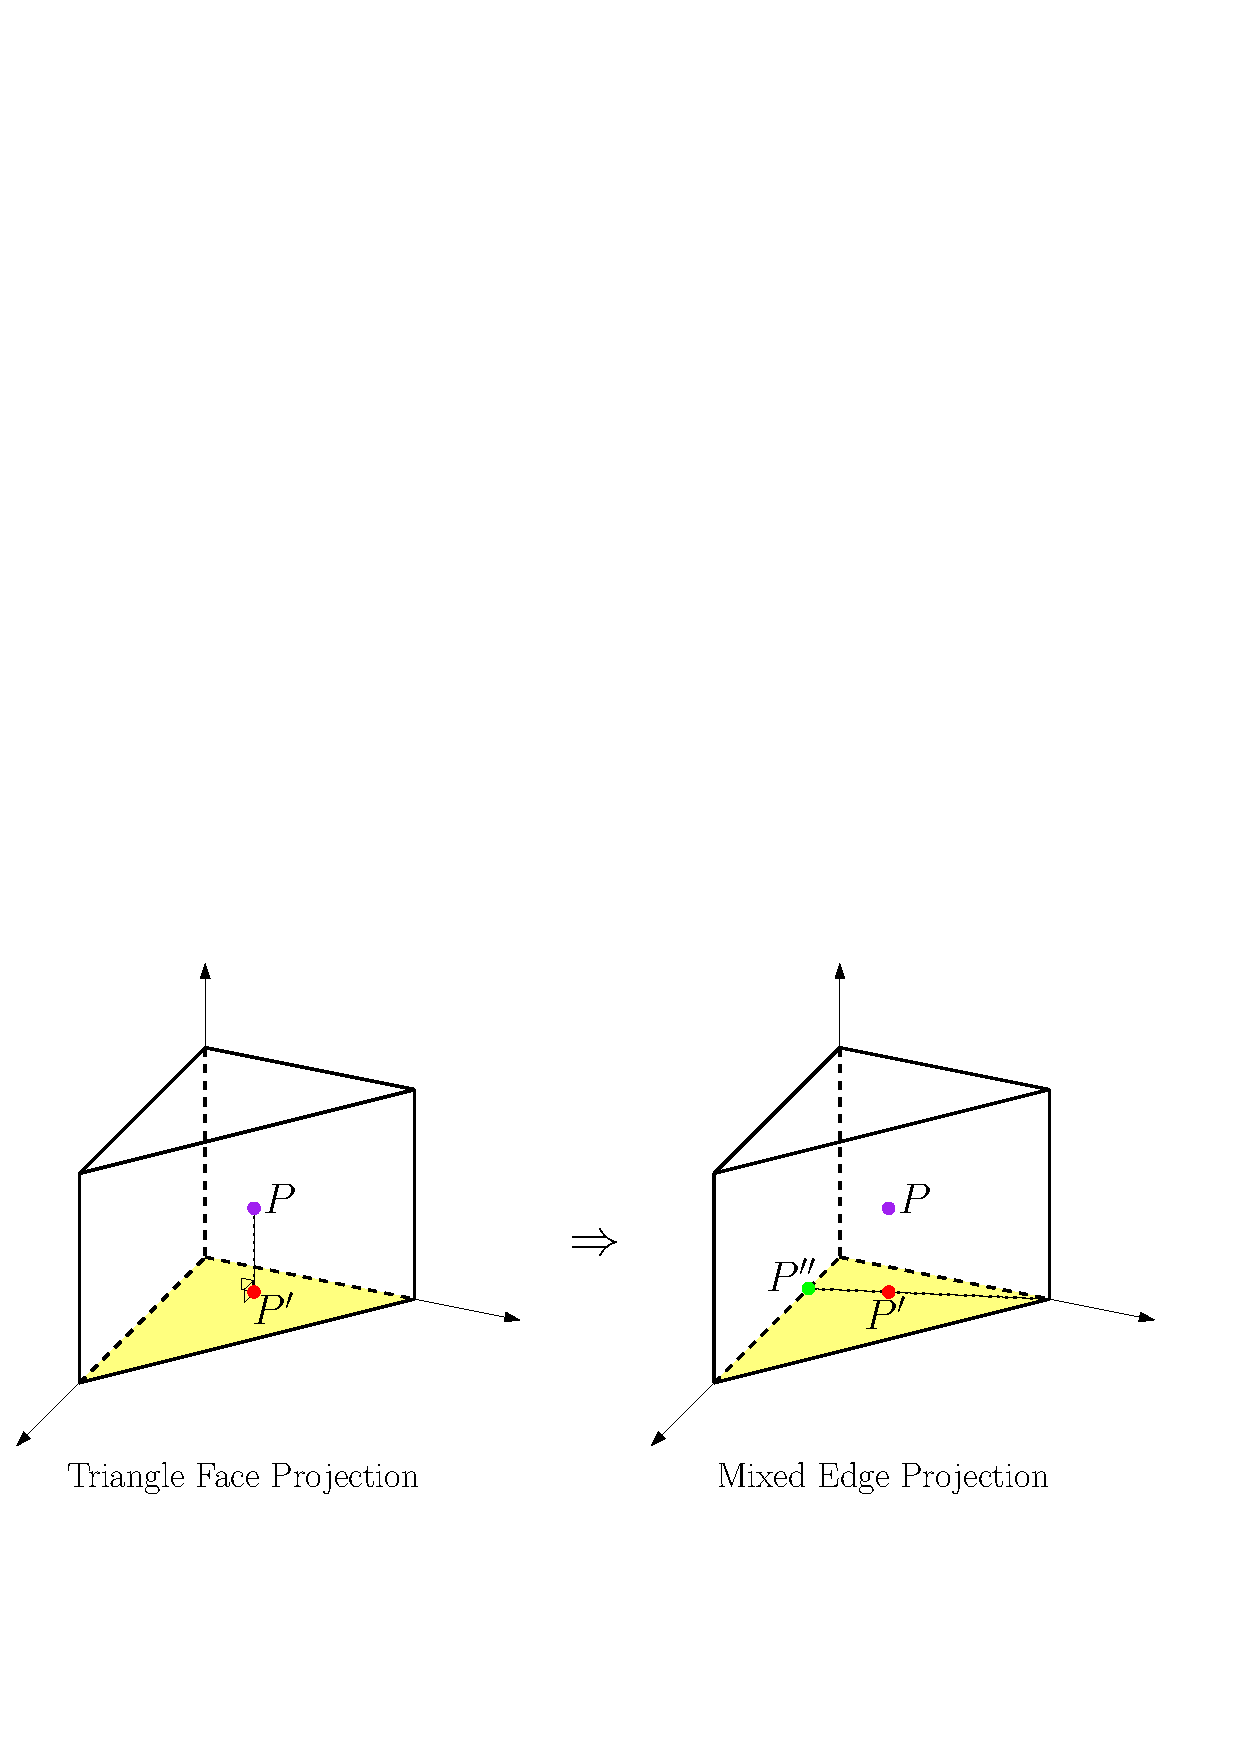
\includegraphics[scale=0.6]{./figures/PrismProjectionTriangle.pdf}
\caption{Triangle face projection from $P$ to $P'$ followed by a mixed edge projection from $P'$ to $P''$.}
\label{fig:PrismProjectionTriangle}
\end{center}
\end{figure}

%Let $\vec{\nu}_{ab}(x)=(\nu_a(x),\nu_b(x))$. 
The shape functions with their gradient are
\begin{equation}
	\begin{aligned}	
		\phi_i^\mathrm{e}(x,z)&=\mu_c(z)\phi_i^\E(\vec{\nu}_{ab}(x))\,,\\
		\nabla\phi_i^\mathrm{e}(x,z)&=\mu_c(z)\nabla\phi_i^\E(\vec{\nu}_{ab}(x))+\phi_i^\E(\vec{\nu}_{ab}(x))\nabla\mu_c(z)\,,
	\end{aligned}\label{eq:PrismH1mixededges}
\end{equation}
where $i=2,\ldots,p$, $0\leq a<b\leq2$, and $c=0,1$. 
There are $p-1$ shape functions for each mixed edge, for a total of $6(p-1)$ mixed edge functions.

%At the edge itself, $\mu_c=1$ and $\vec{\nu}_{ab}(x)$ takes the form $\vec{\mu}_{01}(x_d)$ for some $d=1,2$, so the shape function takes desired $H^1$ edge standard form, $\phi_i^\E(\vec{\mu}_{01}(x_d))$.
%As expected, there is a linear edge blending towards the adjacent quadrilateral face, given by $\mu_c(z)$, and the known triangle edge blending towards the adjacent triangle face, naturally included within $\phi_i^\E$.
%The vanishing trace properties are inherited and easily seen to be satisfied. 


%We consider first the case of the bottom horizontal edges (corresponding to $ \mu_0=1$) with orientation $\mathrm{o}=0$. Recall the triangle edge bubbles (for the $0-1$ edge of the triangle) are given as $\phi^{\mathrm{E}}_{i}(\nu_0(x,y),\nu_1(x,y))$ with $i=2,\cdots,p$ and $p$ being the edge order. The (bottom) horizontal edge shape function for the prism in this case is: \begin{equation}\phi^{e}_i(x,y,z)=\phi^{\mathrm{E}}_{i}(\nu_0(x,y),\nu_1(x,y))\mu_0(z). \nonumber \end{equation}The full set of all prismatic edge shape functions are given as \begin{equation}\phi_i^{\mathrm{E}}(\nu_a,\nu_b)\mu_{c}(z)\nonumber\end{equation} with $a<b \in \{0,1,2\}$ and where $c=1$ corresponds to the top edges and $c=0$ to the bottom edges and $i=2\ldots,p$.

%By the very construction, we see that these edge shape functions vanish at the approprite edges, i.e., for appropriate $a,b$, we see that the product $\phi_i^{\mathrm{E}}(\nu_a,\nu_b)\mu_{m}(z)$ vanishes on all edges except on edge $a-b$.
%\paragraph{Orientation Considerations}
%As before, taking into account orientations, we denote by $\phi_i^{\mathrm{E},\mathrm{o}}(\cdot)$ to indicate that the triangle edges have orientation $\mathrm{o}$. For instance, for the bottom triangle face, we have, \begin{equation}
% \phi_i^{\mathrm{E},\mathrm{o}}(\nu_0,\nu_1)\mu_{0}(z) = \phi_i^{\mathrm{E},\mathrm{o}}(\nu_1,\nu_0)\mu_{0}(z),\end{equation}
% where $\phi_i^{\mathrm{E},\mathrm{o}}(\nu_1,\nu_0)$ is the oriented $0-1$ triangle edge shape function.

\paragraph{\texorpdfstring{$H^1$}{H1} Quadrilateral Edges.}
These are the tensor product of $H^1$ triangle vertex shape functions with the 1D $H^1$ edge functions. 
For edge 03, the shape functions are
\begin{equation*}
	\phi_i^\mathrm{e}(x,z)=\underbrace{\nu_0(x)}_{\text{blend}}
		\underbrace{\phi_i^\E(\underbrace{\mu_0(z),\mu_1(z)}_{\text{project}})}_{\text{evaluate}}\,,
			%=\nu_0(x)[L_i](\mu_0(z),\mu_1(z))=\nu_0(x)L_i(z)\,.
\end{equation*}
for $i=2,\ldots,p$.
As expected, there is a linear edge blending towards both of the adjacent quadrilateral faces, given by $\nu_0(x)$, while all other trace properties are also inherited.
%In this case the projected 1D affine coordinates are simply $(\mu_0(z),\mu_1(z))$ and the projection is
The implied projection is simply
\begin{equation*}
	(x_1,x_2,z)\;\longmapsto\;(\textstyle{\frac{x_1}{1-x_2}},0,z)\;\longmapsto\;(0,0,z)\,.
\end{equation*}
It consists of finding the intersection $P'''=(0,0,z)$ of the edge with the normal plane passing through the original point $P=(x_1,x_2,x_3)$. 
Alternaltively it can be interpreted as a two step projection.
This is illustrated in Figure \ref{fig:PrismProjectionQuad}.

\begin{figure}[!ht]
\begin{center}
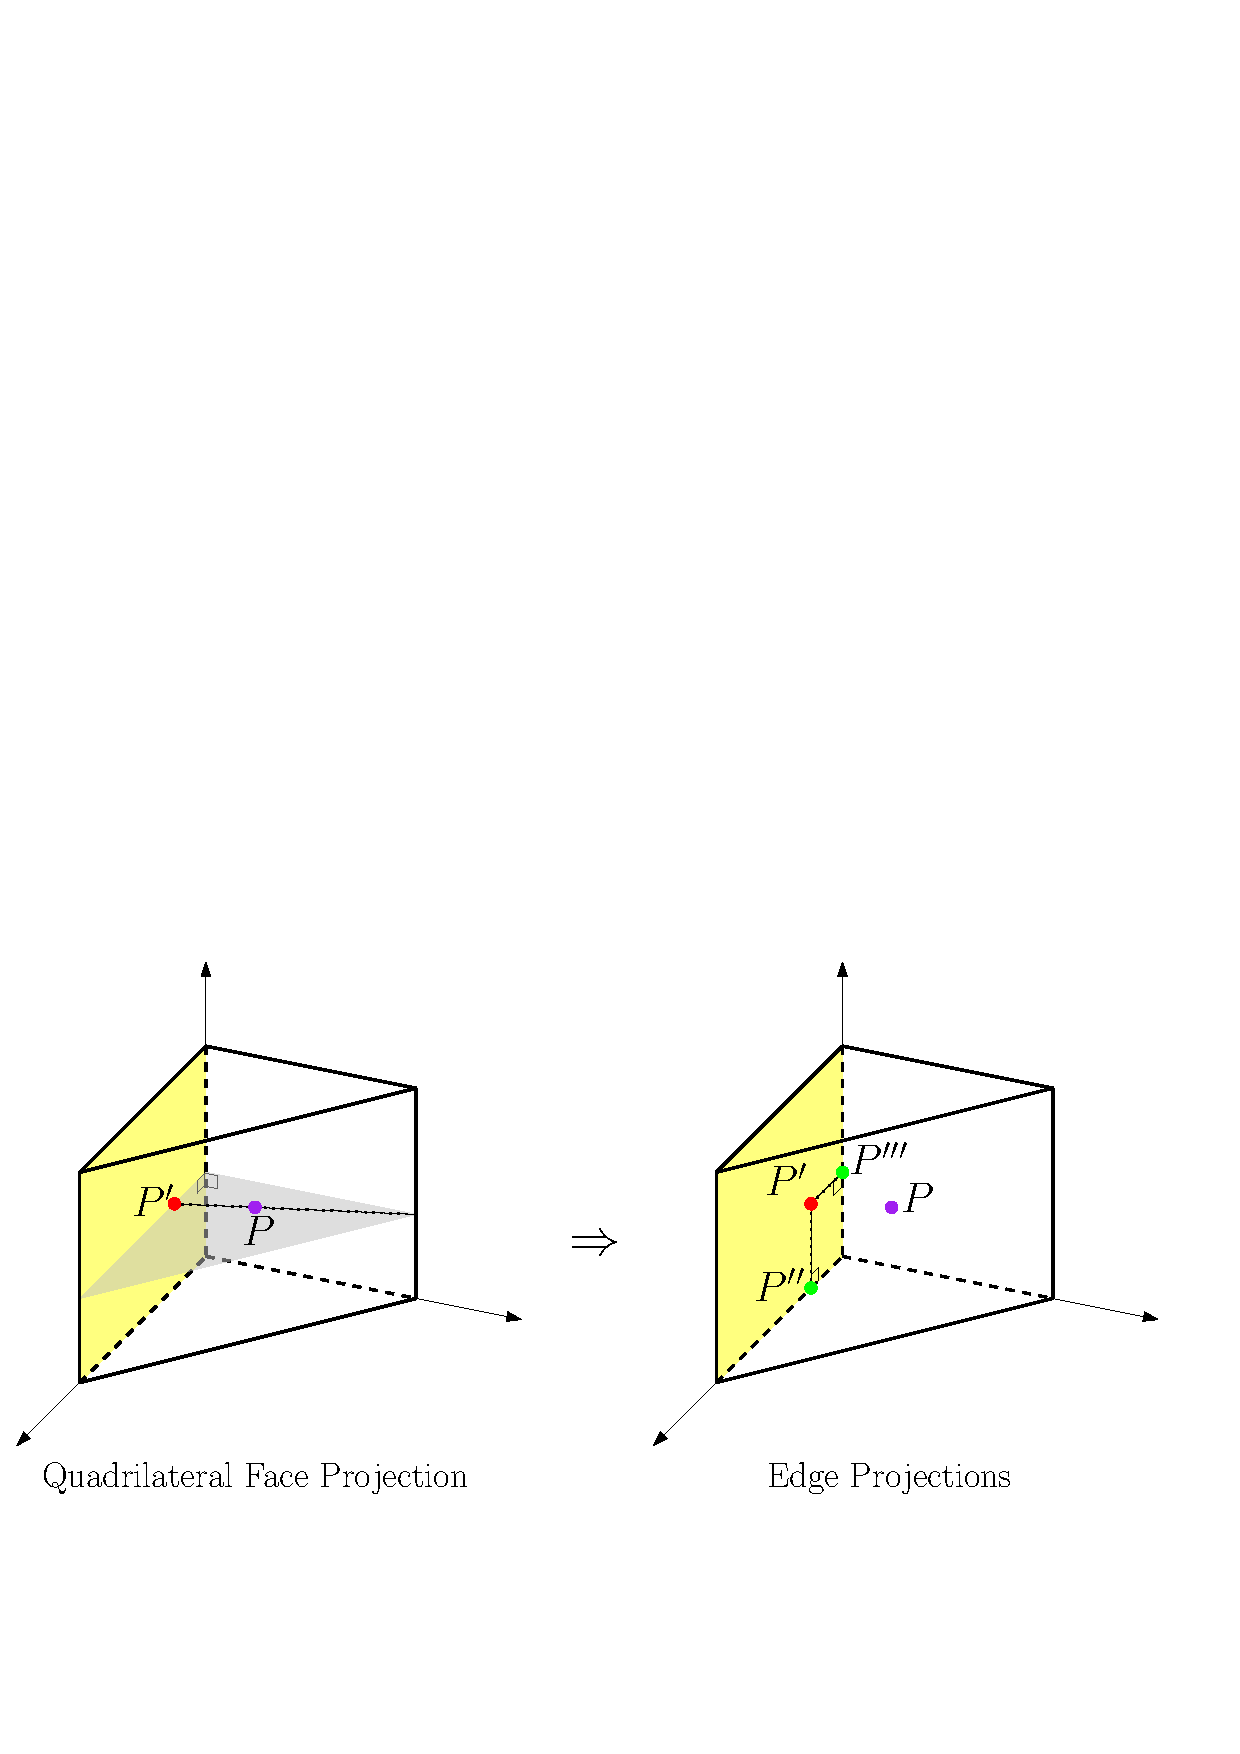
\includegraphics[scale=0.6]{./figures/PrismProjectionQuad.pdf}
\caption{Quadrilateral face projection from $P$ to $P'$ followed by a mixed edge projection from $P'$ to $P''$ and a quadrilateral edge projection from $P'$ to $P'''$.}
\label{fig:PrismProjectionQuad}
\end{center}
\end{figure}

%With $\vec{\mu}_{01}(z)=(\mu_0(z),\mu_1(z))$, the shape functions with their gradients are
The shape functions and their gradient are
\begin{equation}
	\begin{aligned}	
		\phi_i^\mathrm{e}(x,z)&=\nu_a(x)\phi_i^\E(\vec{\mu}_{01}(z))\,,\\
		\nabla\phi_i^\mathrm{e}(x,z)&=\nu_a(x)\nabla\phi_i^\E(\vec{\mu}_{01}(z))+\phi_i^\E(\vec{\mu}_{01}(z))\nabla\nu_a(x)\,,
	\end{aligned}\label{eq:PrismH1quadedges}
\end{equation}
where $i=2,\ldots,q$ and $a=0,1,2$. 
There are $q-1$ shape functions for each quadrilateral edge, for a total of $3(q-1)$ quadrilateral edge functions.

%At the edge itself, where $\nu_a=1$, the shape function takes desired $H^1$ edge standard form $\phi_i^\E(\vec{\mu}_{01}(z))$.
%As expected, there is a linear edge blending towards both of the adjacent quadrilateral faces, given by $\nu_a(x)$.
%Again, the vanishing trace properties are easily inherited. 


%the case of the edge passing through vertex $0$ where the 1D bubbles are oriented with orientation $o=0$. 
%We thus have\begin{equation}\phi_{i}^{e}(x,y,z)=\phi_{i}^{\mathrm{E}}(\mu_0(z),\mu_1(z))\nu_0(x,y)\nonumber \end{equation}with $i=2,\cdots,p$.
%The complete set of all edge shape functions is \begin{equation}\phi_{i}^{e}(x,y,z)=\phi_{i}^{\mathrm{E}}(\mu_0(z),\mu_1(z))\nu_a(x,y) \end{equation}and $a=0,1,2$
%As was the case with shared edges, these also satisfy the appropriate vanishing properties by construction.
%
%\paragraph{Orientation Considerations}
%As before, taking into account orientation, consider the $0-1$ edge. The complete set of vertical edge shape functions is given as $\phi_i^{\mathrm{E},\mathrm{o}}(\mu_{0},\mu_{1})\nu_a(x,y)$, where $\phi_i^{\mathrm{E},\mathrm{o}}(\cdot)$ indicates that the 1D segment has orientation $\mathrm{o}$.

\subsubsection{\texorpdfstring{$H^1$}{H1} Faces} 
%Here again, we have two sets of face shape functions, those that correspond to the horizontal (triangle) faces and those that correspond to the vertical (rectangular) faces.

\paragraph{\texorpdfstring{$H^1$}{H1} Triangle Faces.} 
These are tensor products of $H^1$ triangle face bubbles and 1D $H^1$ vertex shape functions. 
%As before, we first consider the bottom ($\mu_0=1$) triangle face with orientation $\mathrm{o}=0$. 
%To begin, first consider face 012 as an example. The shape functions would be of the form
For instance, for face 012 the shape functions are
\begin{equation*}
	\phi_{ij}^\mathrm{f}(x,z)=\underbrace{\mu_0(z)}_{\text{blend}}
		\underbrace{\phi_{ij}^\Tri(\underbrace{\nu_0(x),\nu_1(x),\nu_2(x)}_{\text{project}})}_{\text{evaluate}}\,,
\end{equation*}
for $i\geq2$ and $j\geq1$.
The trace properties are trivially inherited from each of the components.
The triangle face projection is illustrated in Figure \ref{fig:PrismProjectionTriangle} and consists of finding the intersection $P'=(x_1,x_2,0)$ of the face with the normal line passing through the original point $P=(x_1,x_2,x_3)$.
%The projected 2D affine coordinates are simply $(\nu_0,\nu_1,\nu_2)$, so that the projection is
%\begin{equation*}
%	(x_1,x_2,z)\;\longmapsto\;(x_1,x_2,0)\,.
%\end{equation*}
%This is obtained by finding the intersection $P'=(x_1,x_2,0)$ of the face with the normal line passing through the original point $P=(x_1,x_2,x_3)$. It is shown in Figure \textit{add Figure}.

%Given the triangle face function $\phi_{ij}^{\Tri}(\nu_0(x,y),\nu_1(x,y),\nu_2(x,y))$, with $i \geq 2, j \geq 1, i+j=2, \ldots, p$ and the 1D vertex shape function $\mu_1(z)$ we see that the (bottom) horizontal face shape function of the prism is\begin{equation}\phi_{ij}^f(x,y,z) = \phi_{ij}^{\Tri}(\nu_0(x,y),\nu_1(x,y),\nu_2(x,y))\mu_1(z).\end{equation}
%Note that since these are essentially triangle bubbles tensored with 1D vertex functions, they vanish on the boundary of the triangle faces by construction.
%Let $\vec{\nu}_{012}(x)=(\nu_0(x),\nu_1(x),\nu_2(x))$. 
In general, the shape functions and their gradient are
\begin{equation}
	\begin{aligned}	
		\phi_{ij}^\mathrm{f}(x,z)&=\mu_c(z)\phi_{ij}^\Tri(\vec{\nu}_{012}(x))\,,\\
		\nabla\phi_{ij}^\mathrm{f}(x,z)&=\mu_c(z)\nabla\phi_{ij}^\Tri(\vec{\nu}_{012}(x))
			+\phi_{ij}^\Tri(\vec{\nu}_{012}(x))\nabla\mu_c(z)\,,
	\end{aligned}\label{eq:PrismH1TriFace}
\end{equation}
where $i\geq2$, $j\geq1$, $n=i+j=3,\ldots,p$, and $c=0,1$. 
As with any $H^1$ triangle face, there are $\frac{1}{2}(p-1)(p-2)$ shape functions per face, for a total of $(p-1)(p-2)$ triangle face  functions.

%The shape functions are compatible with neighboring triangle faces, since at the face, where $\mu_c=1$, they are of the form $\phi_{ij}^\Tri(\nu_0(x),\nu_1(x),\nu_2(x))$, which is the $H^1$ standard form for triangle faces. The other vanishing properties are naturally inherited from $\mu_c$ and $\phi_{ij}^\Tri$.

%\paragraph{Orientation Considerations}
%Taking into account orientation, the complete set of horizontal face shape functions is given by $\phi_{ij}^{\Tri,\mathrm{o}}(\nu_0,\nu_1,\nu_2)\mu_c(z)$, $c=0,1$ and $\phi_{ij}^{\mathrm{\Tri},\mathrm{o}}(\cdot)$ refers to the triangle face shape function with orientation $\mathrm{o}$. Note that, as given in the triangle section, we permute the arguments $\nu_0,\nu_1,\nu_2$ of $\phi_{ij}^{\Tri}(\cdot,\cdot,\cdot)$ with the $6$ possible permutations of the axes to arrive at the complete set of shape functions.

\paragraph{\texorpdfstring{$H^1$}{H1} Quadrilateral Faces.} 
%The construction of the vertical face shape functions is a bit more involved. We first consider the case of unswapped axes. We have\begin{equation}\phi_{ij}^f(x,y,z) = \phi_{ij}^{\square}(\nu_a,\nu_b,\mu_0,\mu_1),\end{equation}where $a<b \in \{0,1,2\},$ with $i=2,\ldots,p, j=2,\ldots,q.$ The face function $\phi_{ij}^{\square}(\nu_a,\nu_b,\mu_0,\mu_1)$ is as given in the quadrilateral section. Note here that the polynomial order is $p$ for the triangle edge bubbles and $q$ for the 1D bubbles.
The quadrilateral face functions are simply the product $H^1$ triangle edge functions and 1D $H^1$ edge functions, so they conveniently fall into the general definition of $\phi_{ij}^\square$.
For face 0143, they take the form
\begin{equation*}
	\phi_{ij}^\mathrm{f}(x,z)=\phi_{ij}^\square(\vec{\nu}_{01}(x),\vec{\mu}_{01}(z))
		=\underbrace{(\nu_0(x)+\nu_1(x))^i}_{\text{blend}}
			\underbrace{\phi_{ij}^\square\Big(\underbrace{\textstyle{\frac{1}{\nu_0(x)+\nu_1(x)}}
				\vec{\nu}_{01}(x),\vec{\mu}_{01}(z)}_{\text{project}}\Big)}_{\text{evaluate}}\,,
\end{equation*}
where $i=2,\ldots,p$ and $j=2,\ldots,q$.
Clearly, the desired trace properties are inherited.
%Here, there are two pairs of 1D projected affine coordinates. 
%The first one is $(\frac{\nu_0}{\nu_0+\nu_1},\frac{\nu_1}{\nu_0+\nu_1})$, while the second one is simply $(\mu_0(z),\mu_1(z))$. 
%They represent a projection of the form
%\begin{equation*}
%	(x_1,x_2,z)\;\longmapsto\;(\textstyle{\frac{x_1}{1-x_2}},0,z)\,.
%\end{equation*}
The implied projection, already illustrated in Figure \ref{fig:PrismProjectionQuad}, consists of finding the intersection $P'=(\frac{x_1}{1-x_2},0,z)$ of the face with the projecting line lying in the horizontal plane and passing through the original point $P=(x_1,x_2,x_3)$ and the opposite disjoint quadrilateral edge. 

%Let $\vec{\nu}_{ab}(x)=(\nu_a(x),\nu_b(x))$ and $\vec{\mu}_{01}(z)=(\mu_0(z),\mu_1(z))$. 
The shape functions and their gradient are
\begin{equation}
%	\begin{aligned}	
		\phi_{ij}^\mathrm{f}(x,z)=\phi_{ij}^\square(\vec{\nu}_{ab}(x),\vec{\mu}_{01}(z))\,,\qquad\quad
		\nabla\phi_{ij}^\mathrm{f}(x,z)=\nabla\phi_{ij}^\square(\vec{\nu}_{ab}(x),\vec{\mu}_{01}(z))\,,
%	\end{aligned}\label{eq:PrismH1QuadFace}
\end{equation}
where $i=2,\ldots,p$, $j=2,\ldots,q$, and $0\leq a<b\leq2$. 
There are $(p-1)(q-1)$ shape functions per face, leading to a total of $3(p-1)(q-1)$ quadrilateral face functions.

%The shape functions are compatible with neighboring quadrilateral faces. To see this, note that at the quadrilateral face, $\vec{\nu}_{ab}(x)$ takes the form $\vec{\mu}_{01}(x_d)$ for some $d=1,2$. 
%Hence, the shape functions take the $H^1$ standard form for quadrilateral faces, $\phi_{ij}^\square(\vec{\mu}_{01}(x_d),\vec{\mu}_{01}(z))$. 
%Meanwhile, the other vanishing properties are easily seen to be satisfied.

%Again, these vanish on the quadrilateral edges by construction and also on the shared edges due to the vanishing of the 1D bubbles on the shared triangle edge. Thus, the quadrilateral face functions also satisfy the vanishing properties as required.
%\paragraph{Orientation Considerations}
%We now come to the case of swapped axes. In the case of swapped coordinates, the ordering of the edge functions changes.
%Recall the orientation consideration presented earlier in the case of rectangular faces. The case of swapped axes corrsepond to the case $\mathrm{o}=1$. We then have the complete list of face shap functions, given by: \begin{equation}\phi_{ij}^f(x,y,z) = \phi_{ij}^{\square}(\nu_a,\nu_b,\mu_0,\mu_1) = \phi_{i}^{\mathrm{E},\mathrm{o}}(\nu_a,\nu_b)\phi_{j}^{\mathrm{E},\mathrm{o}}(\mu_0,\mu_1),\end{equation}where , $\phi^{\mathrm{E},\mathrm{o}}(\cdot)$ indicates edge shape functions with orientation $\mathrm{o}$ of the triangle element and segment element with the obvious changes in argument.

\subsubsection{\texorpdfstring{$H^1$}{H1} Interior Bubbles} 
The $H^1$ bubble functions are the tensor product of the $H^1$ triangle face functions and 1D $H^1$ edge functions.
Due to their structure, the zero trace properties are trivially satisfied along the whole boundary.
%With $\vec{\nu}_{012}(x)=(\nu_0(x),\nu_1(x),\nu_2(x))$ and $\vec{\mu}_{01}(z)=(\mu_0(z),\mu_1(z))$, they are

The interior bubbles and their gradient are
\begin{equation}
	\begin{aligned}	
		\phi_{ijk}^\mathrm{b}(x,z)&=\phi_{ij}^\Tri(\vec{\nu}_{012}(x))\phi_k^\E(\vec{\mu}_{01}(z))\,,\\
		\nabla\phi_{ijk}^\mathrm{b}(x,z)&=\phi_k^\E(\vec{\mu}_{01}(z))\nabla\phi_{ij}^\Tri(\vec{\nu}_{012}(x))
			+\phi_{ij}^\Tri(\vec{\nu}_{012}(x))\nabla\phi_k^\E(\vec{\mu}_{01}(z))\,,
	\end{aligned}
\end{equation}
where $i\geq2$, $j\geq1$, $n=i+j=3,\ldots,p$, and $k=2,\ldots,q$. 
There are a total of $\frac{1}{2}(p-1)(p-2)(q-1)$ bubble shape functions in $H^1$.

%The vanishing properties are trivially inherited and checked to hold.

%Given the triangle bubble function $\phi_{ij}^{\Tri}(\nu_0,\nu_1,\nu_2) $ and the 1D bubble function $\phi^{\mathrm{E}}_{k}(\mu_{0}(z),\mu_1(z))$ we have \begin{equation}\phi^{b}_{ijk}(x,y,z) = \phi_{ij}^{\Tri}(\nu_0,\nu_1,\nu_2)\phi_k^{\mathrm{E}}(\mu_0,\mu_1).\end{equation}Here, $i\geq2, j\geq1, i+j=2,\ldots,p$ and $k=2,\dots,q$, where $p$ and $q$ are the polynomial order for the triangle face bubble and 1D bubble respectively. Also, we do not worry about the orientation, as the interior bubble functions are not oriented. By the very construction, the bubble functions are nonzero only on the interior of the prism.



\subsection{\texorpdfstring{$H(\mathrm{curl})$}{Hcurl} Shape Functions}

The linearly independent shape functions presented here are shown to belong and span the $H(\mathrm{curl})$ conforming space $(\mathcal{N}^p\otimes\mathcal{P}^q)\times(\mathcal{P}^p\otimes\mathcal{P}^{q-1})$, which has dimension $p(p+2)(q+1)+\frac{1}{2}(p+2)(p+1)q$.

%%We begin our discussion of $H(\text{curl})$ shape functions with {$H(\text{curl})$} edge functions.
%The $H(\mathrm{curl})$ conforming finite dimensional space is 
%%The dimension of this space is $p(p+2)(q+1)+\frac{1}{2}(p+2)(p+1)q$.
%The shape functions presented here are shown to lie in that space, and by linear independence, they span the space.
%%To see that the shape functions lie in this space, they will be shown in more explicit form, from which it will

These shape functions, as expected, are composed of combinations of $H^1$ and $H(\mathrm{curl})$ components. 
Intuitively, they involve the affine coordinates and at least $E_i^\E$, $E_{ij}^\Tri$ and $E_{ij}^\square$.
All shape functions continue to respect the logic of projecting, evaluating and blending, and for a given topological entity, the projections are the same as those in $H^1$ (see Figures \ref{fig:PrismProjectionTriangle} and \ref{fig:PrismProjectionQuad}).

%It will be clear that all shape functions lie in $\mathcal{P}^p\otimes\mathcal{P}^q$, which has dimension $\frac{1}{2}(p+2)(p+1)(q+1)$. 
%Moreover, a judicious count of the shape functions constructed in this section will coincide with that dimension, ensuring that the span of these is precisely $\mathcal{P}^{p}\otimes\mathcal{P}^q$.


\subsubsection{\texorpdfstring{$H(\mathrm{curl})$}{Hcurl} Edges}
%As was the case with {$H^1$} edge functions, we consider two cases, the horizontal and vertical edge functions.

\paragraph{\texorpdfstring{$H(\mathrm{curl})$}{Hcurl} Mixed Edges.} 
These are tensor products of triangle $H(\text{curl})$ edge functions and 1D $H^1$ vertex functions.
For example, take edge 01. 
Note that $E_i^\E(\vec{\nu}_{01}(x))$ in three dimensions is a three component vector whose last component is zero, since it is independent of the $z$ coordinate. 
Indeed, if considered in \textit{two} dimensions, it is just the well defined triangle $H(\text{curl})$ edge function. 
As such, it is an element of $\mathcal{N}^p$ (in two dimensions). 
Due to this important fact, the first two components of $E_i^\E$ are denoted by $(E_i^\E(\vec{\nu}_{01}(x)))_x\in\mathcal{N}^p$. 
For this edge, the shape functions are
\begin{equation*}
	\begin{aligned}
		E_i^\mathrm{e}(x,z)&=\mu_0(z)E_i^\E(\vec{\nu}_{01}(x))
			%=\begin{pmatrix}\mu_0(z)(E_i^\E(\vec{\nu}_{01}(x)))_{x_1}\\\mu_0(z)(E_i^\E(\vec{\nu}_{01}(x)))_{x_2}\\0\end{pmatrix}
				=\begin{pmatrix}\mu_0(z)(E_i^\E(\vec{\nu}_{01}(x)))_x\\0\end{pmatrix}
					\in(\mathcal{N}^p\otimes\mathcal{P}^1)\times\{0\}\\
		  &=\underbrace{\mu_0(z)(\nu_0(x)+\nu_1(x))^{i+2}}_{\text{blend}}
    		\underbrace{E_i^\E\Big(\underbrace{\textstyle{\frac{1}{\nu_0(x)+\nu_1(x)}\vec{\nu}_{01}(x)}}_{\text{project}}
    			\Big)}_{\text{evaluate}}\,,
	\end{aligned}
\end{equation*}
for $i=0,\ldots,p-1$.
Hence, $E_i^\mathrm{e}\in(\mathcal{N}^p\otimes\mathcal{P}^q)\times(\mathcal{P}^p\otimes\mathcal{P}^{q-1})$.
For the trace properties, note that over faces 1254 and 0253 both tangential components are zero, since the $z$ component is zero and the tangent to edges 12 and 02 is zero by inheritance of $E_i^\E(\vec{\nu}_{01}(x))$.
In the top face, the tangent is also zero because $\mu_0(z)$ is zero there.
Finally, by construction, over face 012 its tangent is precisely the triangle $H(\text{curl})$ edge shape function $(E_i^\E(\vec{\nu}_{01}(x)))_x$, while over face 0143 its tangent behaves like a quadrilateral $H(\text{curl})$ edge function $\mu_0(z)(E_i^\E(\vec{\mu}_{01}(x_1)))_x$.
%The same will apply to the other mixed edges. 
%As an observation, note the curl of the expression above can be expressed in terms of the two dimensional curl and the one dimensional gradient. For this, denote by $\nabla_x\times(E_i^\E(\nu_0(x),\nu_1(x)))_x$ the 2D curl, and by $\nabla_z\mu_0(z)$ the one dimensional gradient. Then,
%\begin{equation*}
%	\nabla\times E_i^\mathrm{e}=\begin{pmatrix}-\nabla_z\mu_0(E_i^\E(\nu_0,\nu_1))_{x_2}\\\nabla_z\mu_0(E_i^\E(\nu_0,\nu_1))_{x_1}\\
%			\mu_0\nabla_x\times(E_i^\E(\nu_0,\nu_1))_x\end{pmatrix}\,.
%\end{equation*}

Now, the general shape functions and their curl are
\begin{equation}
	\begin{aligned}	
		E_i^\mathrm{e}(x,z)&=\mu_c(z)E_i^\E(\vec{\nu}_{ab}(x))\,,\\
		\nabla\times E_i^\mathrm{e}(x,z)&=\mu_c(z)\nabla\times E_i^\E(\vec{\nu}_{ab}(x))
			+\nabla\mu_c(z)\times E_i^\E(\vec{\nu}_{ab}(x))\,,
	\end{aligned}
\end{equation}
with $i=0,\ldots,p-1$, $0\leq a<b\leq2$ and $c=0,1$. 
There are $p$ shape functions for each mixed edge, giving a total of $6p$ mixed edge functions.

%At the edge itself, $\mu_c=1$ and $\vec{\nu}_{ab}(x)$ takes the form $\vec{\mu}_{01}(x_d)$ for some $d=1,2$, so the shape function takes the form $E_i^\E(\vec{\mu}_{01}(x_d))$, whose (tangential) trace is the $L^2$ edge standard form $[P_i](\vec{\mu}_{01}(x_d))$.
%As before, there is a linear edge blending towards the adjacent quadrilateral face, given by $\mu_c(z)$, and the known triangle edge blending towards the adjacent triangle face, naturally included within $E_i^\E$. 
%The remaining vanishing trace properties are easily seen to be inherited.

%Recall the $H(\text{curl})$ edge shape functions for the triangle (with edge ($\nu_{0},\nu_{2}) $) are given as $E_i^{e}(x,y)=E_{i}^{\mathrm{E}}(\nu_{0},\nu_{2}), i\leq p-1$ (assuming orientation $\mathrm{o}=0$). Since $E^e_{i}(x,y)$ is a vector field, it will be convenient to write it in coordinates where $E^\mathrm{E}_{i,1}(\cdot)$ and $E^\mathrm{E}_{i,2}(\cdot)$ are the components of $E^e_{i}(\cdot)$. The horizontal $H(\text{curl})$ edge shape functions are given as:

%\begin{equation} E_{i}^{e}(x,y,z) = \left(
%\begin{array}{c}
%E_{i,1}^{\mathrm{E}}(\nu_{0},\nu_{1})\,\mu_{0}(z)\\
%\\
%E_{i,2}^{\mathrm{E}}(\nu_{0},\nu_{1})\,\mu_{0}(z)\\
%\\
%0 \\
%\end{array}
%\right),
%\nonumber
%\end{equation}
%\\
%\begin{equation} \nabla\times E_{i}^{e}(x,y,z) = \left(
%\begin{array}{c}
%-E_{i,2}^{\mathrm{E}}(\nu_{0},\nu_{1})\,(\nabla \mu_{0}(z))_{,3}\\
%\\
%E_{i,1}^{\mathrm{E}}(\nu_{0},\nu_{1})\,(\nabla \mu_{0}(z))_{,3}\\
%\\
%\nabla \times (E_{i,1}^{\mathrm{E}},E_{i,2}^{\mathrm{E}})\,\mu_{0}(z) \\
%\end{array}
%\right),
%\nonumber
%\end{equation}
%where the $\nabla \times$ is interpreted in 3D and $(\nabla \mu_{0}(z))_{,3}$ denotes the third component of the gradient computed in 3D.
%We can write the above equations compactly by noting \begin{equation}E_{i}^{e}(x,y,z) = E_{i}^{\mathrm{E}}(\nu_{0},\nu_{1})\mu_{0}(z)\nonumber \end{equation} where we interpret $E_{i}^{\mathrm{E}}(\nu_{0},\nu_{1})$ and $\mu_{0}(z)$ as appropriate 3D vectors, so that we have
%\begin{equation}
%\nabla\times E_{i}^{e}(x,y,z)=\mu_0(z)\nabla \times(E_{i}^{\mathrm{E}}(\nu_{0},\nu_{1}))+ \nabla \mu_0(z)\times E_{i}^{\mathrm{E}}(\nu_{0},\nu_{1}),
%\nonumber \end{equation}
%where we interpret $\nabla \times (E_{i}^{\mathrm{E}}(\nu_{0},\nu_{1}))$ as $(\nabla \times(E_{i,1}^{\mathrm{E}}(\cdot),E_{i,2}^{\mathrm{E}}(\cdot)),0) $ the gradient $\nabla\mu_{0}(z)$ as the vector $(0,0,\mu^\prime_{0}(z))$. Again, the functions satisfy the vanishing properties by construction, i.e., the edge function corresponding to edge $0-1$ vanishes on all edges except edge $0-1$. The complete family of (unoriented) $H(\text{curl})$ mixed edge shape functions is given as \begin{equation} E_{i}^{e}(x,y,z) = E_{i}^{\mathrm{E}}(\nu_{a},\nu_{b})\mu_{c}(z)
%\end{equation}
%and 
%\begin{equation}
%\nabla\times E_{i}^{e}(x,y,z)=\mu_c(z)\nabla \times (E_{i}^{\mathrm{E}}(\nu_{a},\nu_{b}))+ \nabla \mu_c(z)\times E_{i}^{\mathrm{E}}(\nu_{a},\nu_{b}),
%\end{equation}
%where $0 \leq a \leq b \leq 2$ and $c=0,1$.
%\paragraph{Orientation Considerations}
%As we saw earlier, to incorporate orientations to the $0-1$ edge of the bottom face, we modify the above equations as \begin{equation}E_{i}^{e}(x,y,z) = E_{i}^{\mathrm{E},\mathrm{o}}(\nu_{0},\nu_{1})\mu_{0}(z).\end{equation}
%The orientation of other faces similarly follows. 

\paragraph{\texorpdfstring{$H(\mathrm{curl})$}{Hcurl} Quadrilateral Edges.} 
%These are tensor products of triangle $H^{1}$ vertex shape functions and 1D $L^2$ shape functions. Considering again the orientation $\mathrm{o}=0$ case of the quadrilateral edge passing through vertex $0$, we have, in coordinates:
These are tensor products of triangle $H^1$ vertex shape functions and $E_i^\E(\vec{\mu}_{01}(z))$, which act as 1D $H(\mathrm{curl})$ functions (even though these do not formally exist for the segment element).
For instance, take edge 03. 
Now, $E_i^\E(\vec{\mu}_{01}(z))$ in three dimensions is a three component vector whose first two components are zero, since it is only dependent on the $z$ coordinate. 
Indeed, if considered in \textit{one} dimension, it is just a segment $L^2$ function belonging to $\mathcal{P}^{q-1}$. 
This last component of $E_i^\E$ is denoted by $(E_i^\E(\vec{\mu}_{01}(z)))_z\in\mathcal{P}^{q-1}$. 
For this edge, the shape functions are
\begin{equation*}
	E_i^\mathrm{e}(x,z)=\underbrace{\nu_0(x)}_{\text{blend}}
			\underbrace{E_i^\E(\underbrace{\vec{\mu}_{01}(z)}_{\text{project}})}_{\text{evaluate}}
		=\begin{pmatrix}0\\0\\\nu_0(x)(E_i^\E(\vec{\mu}_{01}(z)))_{z}\end{pmatrix}
			\in\{0\}\times\{0\}\times(\mathcal{P}^1\otimes\mathcal{P}^{q-1})\,,
\end{equation*}
for $i=0,\ldots,q-1$.
Clearly $E_i^\mathrm{e}\in(\mathcal{N}^p\otimes\mathcal{P}^q)\times(\mathcal{P}^p\otimes\mathcal{P}^{q-1})$.
The trace properties follow easily for the triangle faces, since the vector field points normal to those faces, while in the nonadjacent quadrilateral face 1254 it is zero due to $\nu_0(x)$ being zero.
In the adjacent faces, $E_i^\E(\vec{\mu}_{01}(z))$ is unaffected by the restictions (it is already tangent to the faces and independent of $x$), so the tangential trace is a quadrilateral $H(\text{curl})$ edge function simply because the restriction of $\nu_0(x)$ is a linear blending function over that face.

In view of \eqref{eq:Hcurl1Dspecialcase}, the shape functions and their curl are
\begin{equation}
%	\begin{aligned}	
		E_i^\mathrm{e}(x,z)=\nu_a(x)E_i^\E(\vec{\mu}_{01}(z))\,,\qquad\quad
		\nabla\times E_i^\mathrm{e}(x,z)=\nabla\nu_a(x)\times E_i^\E(\vec{\mu}_{01}(z))\,,
%	\end{aligned}
\end{equation}
with $i=0,\ldots,q-1$, and $a=0,1,2$. 
There are $q$ shape functions for each quadrilateral edge, for a total of $3q$ quadrilateral edge functions.

%%%%At the edge itself, where $\nu_a=1$, the shape function takes desired $H(\mathrm{curl})$ edge standard form $E_i^\E(\vec{\mu}_{01}(z))$.
%%%%As expected, there is a linear edge blending towards both of the adjacent quadrilateral faces, given by $\nu_a(x)$.
%%%%Again, the vanishing trace properties are easily inherited. 

%\begin{equation} E_{i}^e(x,y,z) = \left(
%\begin{array}{c}
%0\\
%\\
%0\\
%\\
%\nu_0(x,y)\,E_{i,3}^{\mathrm{E}}(\mu_0,\mu_1) \\
%\end{array}
%\right),
%\nonumber
%\end{equation}
%\\
%\begin{equation} \nabla\times E_{i}^{e}(x,y,z) = \left(
%\begin{array}{c}
%\frac {\partial\nu_0(x,y)}{\partial y}\,E_{i,3}^{\mathrm{E}}(\mu_0,\mu_1)\\
%\\
%-\frac {\partial\nu_0(x,y)}{\partial x}\,E_{i,3}^{\mathrm{E}}(\mu_0,\mu_1)\\
%\\
%0 \\
%\end{array}
%\right),
%\nonumber
%\end{equation}
%so that we have
%\begin{equation}
% E_{i}^e(x,y,z) = \nu_0(x,y) E_i^{\mathrm{E}}(\mu_0,\mu_1)
%\nonumber
%\end{equation}
%and
%\begin{equation}
%\nabla\times E_{i}^{e}(x,y,z)=\nabla\nu_0(x,y)\times E_i^{\mathrm{E}}(\mu_0,\mu_1),
%\nonumber
%\end{equation}
%where $i=1,\ldots, p$. Again, we interpret the compact equations appropriately in 3D.
%In the above equation, $\nu_0(x,y)$ is the triangle vertex function corresponding to vertex $0$ and we interpret $\nabla\nu_0(x,y)$ as the three-dimensional gradient. Also, $E_i^{\mathrm{E}}(\mu_0,\mu_1)$ is the $i$-th 1D $L^2$ shape function, $i=1,\cdots,p$. Moreover, the functions satisfy the vanishing properties by construction, i.e., the edge function corresponding to vertex $0$ vanishes on all other edges. For the complete list of all $H(\text{curl})$ quadrilateral edge shape functions, we have  \begin{equation} E_{i}^e(x,y,z) = \nu_a(x,y) E_i^{\mathrm{E}}(\mu_0,\mu_1)
%\end{equation}
%and 
%\begin{equation}
%\nabla\times E_{i}^{e}(x,y,z)=(\nabla\nu_a(x,y)\times E_i^{\mathrm{E}}(\mu_0,\mu_1),
%\end{equation}
%where $a=0,1,2$.
%\paragraph{Orientation Considerations}
%As is usual, after incorporating orientations, the modified equations (for the edge passing through vertext $0$) are:\begin{equation} E_{i}^e(x,y,z) = \nu_a(x,y) E_{i}^{\mathrm{E},\mathrm{o}}(x,y,z)
%\end{equation}

\subsubsection{\texorpdfstring{$H(\mathrm{curl})$}{Hcurl} Faces}
%We now consider {$H(\text{curl})$} face shape functions. As was the case with {$H^1$} face functions, we consider two cases, the horizontal (triangle) and vertical(rectangular) face functions.

\paragraph{\texorpdfstring{$H(\mathrm{curl})$}{Hcurl} Triangle Faces.} 
These are tensor products of triangle $H(\text{curl})$ face functions and $H^1$ vertex shape functions. 
As usual, there are two families. 
Proceeding as with $H(\text{curl})$ mixed edge functions, it follows the shape functions lie in $(\mathcal{N}^p\otimes\mathcal{P}^q)\times(\mathcal{P}^p\otimes\mathcal{P}^{q-1})$ and that the trace properties are satisfied.
%They will also be naturally compatible at the faces themselves, and vanish at the other faces. 
As accustomed, there are $p(p-1)$ functions per triangle face, and a grand total of $2p(p-1)$ triangle face functions.

\subparagraph{Family I:} 
The shape functions and their curl are
\begin{equation}
	\begin{aligned}
		E_{ij}^{\mathrm{f}}(x,z)&=\mu_c(z)E_{ij}^\Tri(\vec{\nu}_{012}(x))\,,\\
		\nabla\times E_{ij}^{\mathrm{f}}(x,z)&=\mu_c(z)\nabla\times E_{ij}^\Tri(\vec{\nu}_{012}(x))
			+\nabla\mu_c(z)\times E_{ij}^\Tri(\vec{\nu}_{012}(x))\,,
	\end{aligned}
\end{equation}
for $i\geq0$, $j\geq1$, $n=i+j=1,\ldots,p-1$, and $c=0,1$. 
For every face, there are $\frac{1}{2}p(p-1)$ functions in this family.

\subparagraph{Family II:}
The shape functions and their curl are
\begin{equation}
	\begin{aligned}
		E_{ij}^{\mathrm{f}}(x,z)&=\mu_c(z)E_{ij}^\Tri(\vec{\nu}_{120}(x))\,,\\
		\nabla\times E_{ij}^{\mathrm{f}}(x,z)&=\mu_c(z)\nabla\times E_{ij}^\Tri(\vec{\nu}_{120}(x))
			+\nabla\mu_c(z)\times E_{ij}^\Tri(\vec{\nu}_{120}(x))\,,
	\end{aligned}
\end{equation}
for $i\geq0$, $j\geq1$, $n=i+j=1,\ldots,p-1$, and $c=0,1$.
Note the fact that the entries are $\vec{\nu}_{120}(x)$ as opposed to $\vec{\nu}_{012}(x)$.
For every face, there are $\frac{1}{2}p(p-1)$ functions in this family.


%Recall that (one family of) the triangle $H(\text{curl})$ bubbles are given as $E_{ij}^{f}(x,y)=E_{ij}^{\Tri}(\nu_0,\nu_1,\nu_2)$ with $ i\geq0, j\geq1,i + j = 1,\cdots, p-1.$ Thus, the horizontal $H(\text{curl})$ face shape functions are (as before, in coordinates and $c=0$, i.e., the bottom triangle face)
%
%\begin{equation} E_{ij}^{f}(x,y,z) = \left(
%\begin{array}{c}
%E_{ij,1}^{\Tri}(\nu_0,\nu_1,\nu_2)\,\mu_{0}(z)\\
%\\
%E_{ij,2}^{\Tri}(\nu_0,\nu_1,\nu_2)\,\mu_{0}(z)\\
%\\
%0 \\
%\end{array}
%\right),
%\nonumber
%\end{equation}
%\\
%\begin{equation} \nabla \times E_{ij}^{f}(x,y,z) = \left(
%\begin{array}{c}
%-E_{ij,2}^{\Tri}(\nu_0,\nu_1,\nu_2)\,(\nabla \mu_0(z))_{,3}\\
%\\
%E_{ij,1}^{\Tri}(\nu_0,\nu_1,\nu_2)\,(\nabla \mu_0(z))_{,3}\\
%\\
%\nabla \times (E_{ij,1}^{\Tri},E_{ij,2}^{\Tri})\,\mu_0(z) \\
%\end{array}
%\right),
%\nonumber
%\end{equation}
%so that we have
%\begin{equation} E_{ij}^{f}(x,y,z) = E_{ij}^{\Tri}(\nu_0,\nu_1,\nu_2)\mu_{0}(z)\nonumber \end{equation}
%and 
%\begin{equation}
%\nabla \times E_{ij}^{f}(x,y,z)=\mu_0(z)\nabla \times(E_{ij}^{\Tri}(\nu_0,\nu_1,\nu_2))+\nabla\mu_0(z) \times E_{ij}^{\Tri}(\nu_0,\nu_1,\nu_2),
%\nonumber \end{equation}
%where we again interpret $\nabla \times(E_{ij}^{\Tri}(\nu_0,\nu_1,\nu_2))$ in 3D and $\nabla\mu_0(z)$ as $(0,0,\mu^\prime_0(z)) $. Also, the functions satisfy the vanishing properties by construction, i.e., the face function corresponding to the bottom triangle face vanishes on the entire boundary of the triangle. The complete set of $H(\text{curl})$ triangle face functions is:
%\begin{equation} E_{ij}^{f}(x,y,z) = E_{ij}^{\Tri}(\nu_0,\nu_1,\nu_2)\mu_{c}(z)\end{equation}
%and
%\begin{equation}
%\nabla \times E_{ij}^{f}(x,y,z)=\mu_c(z)\nabla \times (E_{ij}^{\Tri}(\nu_0,\nu_1,\nu_2))+\nabla\mu_c(z) \times E_{ij}^{\Tri}(\nu_0,\nu_1,\nu_2),
%\end{equation}
%with $c=0,1$.
%\paragraph{Orientation Considerations}
%To obtain orientation embedded functions, we change the orientation of $E_{ij}^{\Tri}(\nu_0,\nu_1,\nu_2)$, i.e, we replace $E_{ij,1}^{\Tri}(\nu_0,\nu_1,\nu_2)$ and $E_{ij,2}^{\Tri}(\nu_0,\nu_1,\nu_2)$  with $E_{ij,1}^{\Tri,\mathrm{o}}(\nu_0,\nu_1,\nu_2)$ and $E_{ij,2}^{\Tri,\mathrm{o}}(\nu_0,\nu_1,\nu_2)$ respectively and the rest of the construction is as above.

\paragraph{\texorpdfstring{$H(\mathrm{curl})$}{Hcurl} Quadrilateral Faces.} 
These are tensor products of $H(\text{curl})$ triangle edge functions and $H^1$ 1D edge shape functions, and viceversa, so that it is clear there are two families. 
Both fall naturally into the general definition of $E_{ij}^\square$.
There are a total of $p(q-1)+q(p-1)$ functions per quadrilateral face, for a grand total of $3(p(q-1)+q(p-1))$ quadrilateral face functions.
%It is worth observing these families separately in a little more detail because they have different forms.
%\footnote{Note that when orientations are being considered, the two families might switch their role, but this is taken care of automatically by the oriented versions of $E_{ij}^{\square_I}$ and $E_{ij}^{\square_{II}}$. See \S\ref{sec:PrismFaceOrientations}.}

\subparagraph{Family I:}
To begin, take for example face 0143. 
The shape functions for the first family are of the form $E_{ij}^\square(\vec{\nu}_{01}(x),\vec{\mu}_{01}(z))$, so proceeding exactly as with the \textit{mixed} edges it is easily shown that it lies in $(\mathcal{N}^p\otimes\mathcal{P}^q)\times\{0\}$ and more importantly that the trace properties hold.
%\begin{equation*}
%	E_{ij}^\mathrm{f}=E_{ij}^{\square_I}(\vec{\nu}_{01},\vec{\mu})
%		=\begin{pmatrix}\phi_j^\E(\vec{\mu})(E_i^\E(\vec{\nu}_{01}))_{x_1}\\[2pt]
%				\phi_j^\E(\vec{\mu})(E_i^\E(\vec{\nu}_{01}))_{x_2}\\[2pt]0\end{pmatrix}
%			=\begin{pmatrix}\phi_j^\E(\vec{\mu})(E_i^\E(\vec{\nu}_{01}))_x\\0\end{pmatrix}
%				\subseteq(\mathcal{N}^p\otimes\mathcal{P}^q)\times\{0\}\,,
%\end{equation*}
%so that $E_{ij}^{\square_I}(\nu_0,\nu_1,\mu_0,\mu_1)\in(\mathcal{N}^p\otimes\mathcal{P}^q)\times(\mathcal{P}^p\otimes\mathcal{P}^{q-1})$.

The general shape functions and their curl are
\begin{equation}
	%\begin{aligned}
		E_{ij}^{\mathrm{f}}(x,z)=E_{ij}^\square(\vec{\nu}_{ab}(x),\vec{\mu}_{01}(z))\,,\qquad\quad
		\nabla\times E_{ij}^{\mathrm{f}}(x,z)=\nabla\times E_{ij}^\square(\vec{\nu}_{ab}(x),\vec{\mu}_{01}(z))\,,
	%\end{aligned}
\end{equation}
for $i=0,\ldots,p-1$, $j=2,\ldots,q$, and $0\leq a<b\leq2$. 
There are $p(q-1)$ shape functions in this family per quadrilateral face.

\subparagraph{Family II:}
Again, taking face 0143 as an example, the second family of shape functions has the form $E_{ij}^\square(\vec{\mu}_{01}(z),\vec{\nu}_{01}(x))$.
This time, proceeding as with \textit{quadrilateral} edges, one can show that the trace properties hold and that the functions lie in $\{0\}\times\{0\}\times(\mathcal{P}^p\otimes\mathcal{P}^{q-1})$.
%To begin, take face 0143. The shape functions are of the form
%\begin{equation*}
%	E_{ij}^\mathrm{f}=E_{ij}^{\square_{II}}(\nu_0,\nu_1,\mu_0,\mu_1)
%		=\begin{pmatrix}0\\0\\\phi_i^\E(\nu_0,\nu_1)(E_j^\E(\mu_0,\mu_1))_{z}\end{pmatrix}
%			\subseteq\{0\}\times\{0\}\times(\mathcal{P}^p\otimes\mathcal{P}^{q-1})\,,
%\end{equation*}
%so that $E_{ij}^{\square_{II}}(\nu_0,\nu_1,\mu_0,\mu_1)\in(\mathcal{N}^p\otimes\mathcal{P}^q)\times(\mathcal{P}^p\otimes\mathcal{P}^{q-1})$.

The general shape functions and their curl are
\begin{equation}
	%\begin{aligned}
		E_{ij}^{\mathrm{f}}(x,z)=E_{ij}^\square(\vec{\mu}_{01}(z),\vec{\nu}_{ab}(x))\,,\qquad\quad
		\nabla\times E_{ij}^{\mathrm{f}}(x,z)=\nabla\times E_{ij}^\square(\vec{\mu}_{01}(z),\vec{\nu}_{ab}(x))\,,
	%\end{aligned}
\end{equation}
for $i=0,\ldots,q-1$, $j=2,\ldots,p$, and $0\leq a<b\leq2$. 
Note the entries are permuted with respect to the first family.
There are $q(p-1)$ shape functions in this family per quadrilateral face.

%These are perhaps the most tricky to implement. We first consider the unswapped case to show the generic construction and then comment on the swapped case. If the coordinate axes are not swapped, we have the following two families of functions.
%\\
%\\
%\textbf{Family I} The first family functions are similar to those
%for horizontal edges except that in the vertical direction we employ now 1D $H^1$ bubbles. We first consider the orientation $\mathrm{o}=0$ case (in coordinates, as before) of the quadrilateral face passing through the bottom $0-1$ triangle face.
%
%
%\begin{equation} E_{ij}^{f}(x,y,z) =  E_{ij}^{\square}(\nu_0,\nu_1, \mu_0,\mu_1) = \left(
%\begin{array}{c}
%E^{\mathrm{E}}_{i,1}(\nu_0,\nu_1)\,\phi^{\mathrm{E}}_{j}(\mu_0,\mu_1)\\
%\\
%E^{\mathrm{E}}_{i,2}(\nu_0,\nu_1)\,\phi^{\mathrm{E}}_{j}(\mu_0,\mu_1)\\
%\\
%0 \\
%\end{array}
%\right),
%\nonumber
%\end{equation}
%\\
%\begin{equation} \nabla \times E_{ij}^{f}(x,y,z) = \nabla E_{ij}^{\square}(\nu_0,\nu_1, \mu_0,\mu_1) = \left(
%\begin{array}{c}
%-E^{\mathrm{E}}_{i,2}(\nu_0,\nu_1)\,(\nabla \phi_j^{\mathrm{E}}(\mu_0,\mu_1))_{,3}\\
%\\
%E^{\mathrm{E}}_{i,1}(\nu_0,\nu_1)\,(\nabla \phi_j^{\mathrm{E}}(\mu_0,\mu_1))_{,3}\\
%\\
%\nabla \times (E^{\mathrm{E}}_{i,1},E^{\mathrm{E}}_{i,2})\,\phi^{\mathrm{E}}_{j}(\mu_0,\mu_1) \\
%\end{array}
%\right),
%\nonumber
%\end{equation}
%We have
%
%\begin{equation} E_{ij}^{f}(x,y,z) =  E_{ij}^{\square}(\nu_0,\nu_1, \mu_0,\mu_1) =  E_{i}^{\mathrm{E}}(\nu_0,\nu_1)\phi^{\mathrm{E}}_{j}(\mu_0,\mu_1)
%\nonumber \end{equation}
%and
%\begin{equation}
%\nabla E_{ij}^{\square}(\nu_0,\nu_1, \mu_0,\mu_1)=\phi^{\mathrm{E}}_{j}(\mu_0,\mu_1)\nabla \times (E^{\mathrm{E}}_{i}(\nu_0,\nu_1)+\nabla\phi^{\mathrm{E}}_{j}(\mu_0,\mu_1)\times E^{\mathrm{E}}_{i}(\nu_0,\nu_1),
%\nonumber
%\end{equation}
%where the interpretation of the above equations and $\nabla \times (E^{\mathrm{E}}_{i}(\nu_0,\nu_1)) $ is in 3D and $\nabla\phi^{\mathrm{E}}_{j}(\mu_0,\mu_1)$ is $(0,0,\frac{d\phi^{\mathrm{E}}_{j}(\mu_0,\mu_1)}{dz}) $. Also,  $ i=1,\ldots p-1, \,j=1,\ldots, q$.
%Here $E^{\mathrm{E}}_{i}(\nu_0,\nu_1)$ is the $i$-th triangle edge shape function and
%$\phi^{\mathrm{E}}_{j}(\mu_0,\mu_1)$ is the $j$-th 1D bubble shape function and $(p,q)$ is the face order. For the complete list of family $I$ face functions, we have \begin{equation} E_{ij}^{f}(x,y,z) =  E_{ij}^{\square}(\nu_a,\nu_b, \mu_0,\mu_1) =  E_{i}^{\mathrm{E}}(\nu_a,\nu_b)\phi^{\mathrm{E}}_{j}(\mu_0,\mu_1)
%\end{equation} and \begin{equation}
%\nabla E_{ij}^{\square}(\nu_a,\nu_b, \mu_0,\mu_1)=\phi^{\mathrm{E}}_{j}(\mu_0,\mu_1)\nabla \times(E^{\mathrm{E}}_{i}(\nu_a,\nu_b)+\nabla\phi^{\mathrm{E}}_{j}(\mu_0,\mu_1)\times E^{\mathrm{E}}_{i}(\nu_a,\nu_b),
%\end{equation}
%with $0 \leq a \leq b \leq 2$.
%\\
%\\
%\textbf{Family II}
%Functions belonging to the second family are similar to those for vertical edges, i.e.,  are the tensor product of triangle $H^1$ edge bubbles with 1D $L^2$ shape functions. We consider the orientation $\mathrm{o}=0$ case first.
%
%
%
%\begin{equation} E_{ij}^{f}(x,y,z) = E_{ij}^{\square}(\nu_0,\nu_1, \mu_0,\mu_1) = \left(
%\begin{array}{c}
%0\\
%\\
%0\\
%\\
%\phi^{\mathrm{E}}_i(\nu_0,\nu_1)\,(E^{\mathrm{E}}_j(\mu_0,\mu_1)_{,3} \\
%\end{array}
%\right),
%\nonumber
%\end{equation}
%\\
%\begin{equation} \nabla \times E_{ij}^{f}(x,y,z) = \nabla \times E_{ij}^{\square}(\nu_0,\nu_1, \mu_0,\mu_1) = \left(
%\begin{array}{c}
%\frac {\partial\phi^{\mathrm{E}}_i(\nu_0,\nu_1)}{\partial y}\,(E^{\mathrm{E}}_j(\mu_0,\mu_1))_{,3}\\
%\\
%-\frac {\partial\phi^{\mathrm{E}}_i(\nu_0,\nu_1)}{\partial x}\,(E^{\mathrm{E}}_j(\mu_0,\mu_1))_{,3}\\
%\\
%0 \\
%\end{array}
%\right),
%\nonumber
%\end{equation}
%so that we have
%
%\begin{equation} E_{ij}^{f}(x,y,z) = E_{ij}^{\square}(\nu_0,\nu_1, \mu_0,\mu_1) = \phi_{i}^{\mathrm{E}}(\nu_0,\nu_1)E_{j}^{\mathrm{E}}(\mu_0,\mu_1)
%\nonumber\end{equation}
%
%\begin{equation}
%\nabla \times E_{ij}^{\square}(\nu_0,\nu_1, \mu_0,\mu_1)=\nabla\phi^{\mathrm{E}}_i(\nu_0,\nu_1) \times (E^{\mathrm{E}}_j(\mu_0,\mu_1)),
%\nonumber \end{equation}
%where $i=1,\ldots, p-1,\, j=1,\ldots,q$ and we interpret $\nabla\phi^{\mathrm{E}}_i(\nu_a,\nu_b)$ as the three-dimensional gradient.
%
%For the complete list of family II face functions we have:\begin{equation} E_{ij}^{f}(x,y,z) = E_{ij}^{\square}(\nu_a,\nu_b, \mu_0,\mu_1) = \phi_{i}^{\mathrm{E}}(\nu_a,\nu_b)E_{j}^{\mathrm{E}}(\mu_0,\mu_1)
%\end{equation}
%and 
%\begin{equation}
%\nabla \times E_{ij}^{\square}(\nu_a,\nu_b, \mu_0,\mu_1)=\nabla\phi^{\mathrm{E}}_i(\nu_a,\nu_b)\times E_{j}^{\mathrm{E}}(\mu_0,\mu_1).
%\end{equation}
%
%
%Both families of functions satisfy the vanishing properties by construction, i.e., the face function corresponding to a quadrilateral face vanishes on the entire boundary of the quadrilateral. This follows by the construction of the face functions.
%
%\paragraph{Orientation Considerations}
%We consider orientations for both families.
%
%For the first family, to account for orientation (considering the face corresponding to the bottom $0-1$ edge) of the triangle faces, we use $E^{\mathrm{E},\mathrm{o}}_{i}(\nu_0,\nu_1)\phi_j^{\mathrm{E},\mathrm{o}}(\mu_0,\mu_1)$ in place of $E^{\mathrm{E}}_{i}(\nu_0,\nu_1)\phi^{\mathrm{E}}_{j}(\mu_0,\mu_1)$ in the above equation.
%
%
%For the second family, to include orientations, as is usual, we replace $\phi_i^{\mathrm{E}}(\nu_0,\nu_1)$ with $\phi_i^{\mathrm{E},\mathrm{o}}(\nu_0,\nu_1)$
%
%We now come to the case of swapped axes. As before, in the case of the swapped axes, the ordering of face shape functions changes. The second family becomes
%first and the loop order in indices $i,j$ changes as well: $ j=1,\ldots,q,\, i=1,\ldots, p-1$.
%Then the first family follows with switched loops in $i,j$ as well.
%As we saw earlier, the case of swapped axes corrsepond to the situation of local and global axes being swapped. We then have the complete list of face shape functions, given by:
%\\
%
%\textbf{Family I}
%\begin{equation} E_{ij}^{f}(x,y,z)  = E_{ij}^{\square,\mathrm{o}}(\nu_0,\nu_1, \mu_0,\mu_1) = E_{i}^{\mathrm{E},\mathrm{o}}(\nu_0,\nu_1)\phi^{\mathrm{E},\mathrm{o}}_{j}(\mu_0,\mu_1)
%\end{equation}
%\\
%
%\textbf{Family II}
%\begin{equation} E_{ij}^{f}(x,y,z) = E_{ij}^{\square,\mathrm{o}}(\nu_0,\nu_1, \mu_0,\mu_1) = \phi_{i}^{\mathrm{E}}(\nu_0,\nu_1)E_{j}^{\mathrm{E}}(\mu_0,\mu_1).
%\end{equation}
%\\

\subsubsection{\texorpdfstring{$H(\mathrm{curl})$}{Hcurl} Interior Bubbles}

There are three families of interior bubble functions.
They involve tensor products of $\phi_i^\E$, $\phi_{ij}^\Tri$, $E_i^\E$ and  $E_{ij}^\Tri$.
The first two families have elements lying in $(\mathcal{N}^p\otimes\mathcal{P}^q)\times\{0\}$, while the last family has elements in $\{0\}\times\{0\}\times(\mathcal{P}^p\otimes\mathcal{P}^{q-1})$.
The trace properties are also satisfied by using similar arguments to those used for the face and edge functions. 
There is a grand total of $p(p-1)(q-1)+\frac{1}{2}(p-1)(p-2)q$ interior bubble functions.


%There are a total of three families of bubble functions. Two of them are naturally induced by $E_{ij}^\Tri$ and $E_{ij}^\Tri}$, while the third family is closely related to $E_{ik}^{\square_{II}}$. 
%The first two families have a total of $p(p-1)(q-1)$ shape functions, while the third family has $\frac{1}{2}(p-1)(p-2)q$ functions.
%For the three families, the vanishing properties are easily seen to be satisfied.

\subparagraph{Family I:}
The shape functions and their curl are
\begin{equation}
	\begin{aligned}	
		E_{ijk}^\mathrm{b}(x,z)&=\phi_k^\E(\vec{\mu}_{01}(z))E_{ij}^\Tri(\vec{\nu}_{012}(x))\,,\\
		\nabla\times E_{ijk}^\mathrm{b}(x,z)&=\phi_k^\E(\vec{\mu}_{01}(z))\nabla\times E_{ij}^\Tri(\vec{\nu}_{012}(x))
			+\nabla\phi_k^\E(\vec{\mu}_{01}(z))\times E_{ij}^\Tri(\vec{\nu}_{012}(x))\,,
	\end{aligned}
\end{equation}
with $i\geq0$, $j\geq1$, $n=i+j=1,\ldots,p-1$, and $k=2,\ldots,q$. 
The family has $\frac{1}{2}p(p-1)(q-1)$ functions.
%As with $H(\text{curl})$ mixed edge functions, it follows the shape functions lie in $(\mathcal{N}^p\otimes\mathcal{P}^q)\times(\mathcal{P}^p\otimes\mathcal{P}^{q-1})$. 

\subparagraph{Family II:}
The shape functions and their curl are
\begin{equation}
	\begin{aligned}	
		E_{ijk}^\mathrm{b}(x,z)&=\phi_k^\E(\vec{\mu}_{01}(z))E_{ij}^\Tri(\vec{\nu}_{120}(x))\,,\\
		\nabla\times E_{ijk}^\mathrm{b}(x,z)&=\phi_k^\E(\vec{\mu}_{01}(z))\nabla\times E_{ij}^\Tri(\vec{\nu}_{120}(x))
			+\nabla\phi_k^\E(\vec{\mu}_{01}(z))\times E_{ij}^\Tri(\vec{\nu}_{120}(x))\,,
	\end{aligned}
\end{equation}
with $i\geq0$, $j\geq1$, $n=i+j=1,\ldots,p-1$, and $k=2,\ldots,q$. 
The only difference with the first family is that the permutation $\vec{\nu}_{120}(x)$ is used instead of $\vec{\nu}_{012}(x)$.
The family has $\frac{1}{2}p(p-1)(q-1)$ functions.
%As with $H(\text{curl})$ mixed edge functions, it follows the shape functions lie in $(\mathcal{N}^p\otimes\mathcal{P}^q)\times(\mathcal{P}^p\otimes\mathcal{P}^{q-1})$.

\subparagraph{Family III:}
Due to \eqref{eq:Hcurl1Dspecialcase}, the shape functions and their curl are
\begin{equation}
	\begin{aligned}	
		E_{ijk}^\mathrm{b}(x,z)&=\phi_{ij}^\Tri(\vec{\nu}_{012}(x))E_k^\E(\vec{\mu}_{01}(z))\,,\\
		\nabla\times E_{ijk}^\mathrm{b}(x,z)&=\nabla\phi_{ij}^\Tri(\vec{\nu}_{012}(x))\times E_k^\E(\vec{\mu}_{01}(z))\,,
	\end{aligned}
\end{equation}
with $i\geq2$, $j\geq1$, $n=i+j=3,\ldots,p$, and $k=0,\ldots,q-1$. 
The family has $\frac{1}{2}(p-1)(p-2)q$ functions.
%As with $E_{ij}^{\square_{II}}(\vec{\nu}_{ab},\vec{\mu})$, it follows the shape functions lie in $(\mathcal{N}^p\otimes\mathcal{P}^q)\times(\mathcal{P}^p\otimes\mathcal{P}^{q-1})$.

%\subsubsection{\boldmath{$H(\text{curl})$} Bubbles} We now consider {$H(\text{curl})$} bubble functions. There are two families of {$H(\text{curl})$} bubble functions. As with other bubble functions, we do not consider orientations for bubbles.
%\\
%
%
%\textbf{Family I}
%The first family is obtained as the tensor product of triangle {$H(\text{curl})$} face functions with 1D $H^1$ bubbles. Recall that (one family of) the triangle $H(\text{curl})$ face functions are given as $E_{ij}^f(x,y) = E^{\Tri}_{ij}(\nu_0,\nu_1,\nu_2)$ with $ i\geq0, j\geq1,i + j = 1,\ldots, p-1$, and $ \phi_k^{\mathrm{E}}(z)$ denotes the 1D $H^1$ bubble. The first family of prism $H(\text{curl})$ bubble function are therefore given by
%
%
%
%\begin{equation} E_{ijk}^{b}(x,y,z)  = \left(
%\begin{array}{c}
%E_{ij,1}^{\Tri}(\nu_0,\nu_1,\nu_2)\phi_k^{\mathrm{E}}(\mu_0,\mu_1)\\
%\\
%E_{ij,2}^{\Tri}(\nu_0,\nu_1,\nu_2)\phi_k^{\mathrm{E}}(\mu_0,\mu_1))\\
%\\
%0 \\
%\end{array}
%\right),
%\end{equation}
%\\
%\begin{equation} \nabla \times E_{ijk}^{b}(x,y,z) = \left(
%\begin{array}{c}
%-E^{\Tri}_{ij,2}(\nu_0,\nu_1,\nu_2)\,(\nabla \phi_{k}^{E}(\mu_0,\mu_1))_{,3}\\
%\\
%E^{\Tri}_{ij,1}(\nu_0,\nu_1,\nu_2)\,(\nabla \phi_{k}^{E}(\mu_0,\mu_1))_{,3}\\
%\\
%\nabla \times (E^{\Tri}_{ij,1},E^{\Tri}_{ij,2})\,\phi^{\mathrm{E}}_{k}(\mu_0,\mu_1) \\
%\end{array}
%\right),
%\end{equation}
%so that we have
%\begin{equation}
%\nabla \times E_{ijk}^{b}(x,y,z)=\phi^{\mathrm{E}}_{k}(\mu_0,\mu_1)\nabla \times (E^{\Tri}_{ij}(\nu_0,\nu_1,\nu_2)+\nabla\phi^{\mathrm{E}}_{k}(\mu_0,\mu_1)\times E^{\Tri}_{ij}(\nu_0,\nu_1,\nu_2),
%\end{equation}
%with $k=2,\cdots,q$ and the usual interpretations of $\nabla\phi^{\mathrm{E}}_{j}(\mu_0,\mu_1)$ and $\nabla \times (E^{\Tri}_{ij}(\nu_0,\nu_1,\nu_2))$. Moreover, by replacing 
%$E_{ij}^{\Tri}(\nu_0,\nu_1,\nu_2)$ with $E_{ij}^{\Tri}(\nu_1,\nu_2,\nu_0)$ we can generate another set of bubble functions based on the above construction.
%\\
%
%\textbf{Family II}
%The second family is obtained as the tensor product of triangle {$H^1$} face functions with 1D $L^2$ functions. Recall that (one family of) the triangle $H^1$ face functions are given as $\phi_{ij}^f(x,y) = \phi^{\Tri}_{ij}(\nu_0,\nu_1,\nu_2)$ with $ i\geq0, j\geq1,i + j = 1,\ldots, p-1$. The second family of prism $H(\text{curl})$ bubble function are therefore given by
%
%
%\begin{equation} E_{ijk}^{b}(x,y,z) = \left(
%\begin{array}{c}
%0\\
%\\
%0\\
%\\
%\phi^{\Tri}_{ij}(\nu_0,\nu_1,\nu_2)\,E_k^{\mathrm{E}}(\mu_0,\mu_1)_{,3} \\
%\end{array}
%\right),
%\end{equation}
%\\
%\begin{equation} \nabla\times E_{ijk}^{b}(x,y,z) = \left(
%\begin{array}{c}
%\frac {\partial\phi^{\Tri}_{ij}(\nu_0,\nu_1,\nu_2)}{\partial y}\,E_k^{\mathrm{E}}(\mu_0,\mu_1)_{,3}\\
%\\
%-\frac {\partial\phi^{\Tri}_{ij}(\nu_0,\nu_1,\nu_2)}{\partial x}\,E_k^{\mathrm{E}}(\mu_0,\mu_1)_{,3}\\
%\\
%0 \\
%\end{array}
%\right),
%\end{equation}
%so that we have
%\begin{equation}
%\nabla\times E_{ijk}^{b}(x,y,z)=\nabla\phi^{\Tri}_{ij}(\nu_0,\nu_1,\nu_2)\times E_k^{\mathrm{E}}(\mu_0,\mu_1),
%\end{equation}
%
%with $i,j\geq0, \, i+j=2,\ldots,p$ and $k=1,\ldots,q$ where $p,q$ are the triangle and 1D orders respectively. Moreover, we have the usual interpretations of $\nabla\phi^{\Tri}_{ij}(\nu_0,\nu_1,\nu_2)$.


\subsection{\texorpdfstring{$H(\mathrm{div})$}{Hdiv} Shape Functions}
The linearly independent shape functions presented here are shown to belong and span the $H(\mathrm{div})$ conforming space $(\mathcal{RT}^p\otimes\mathcal{P}^{q-1})\times(\mathcal{P}^{p-1}\otimes\mathcal{P}^q)$, which has dimension $p(p+2)q+\frac{1}{2}p(p+1)(q+1)$.

As expected, the shape functions are composed of combinations of the lower dimensional $H^1$, $H(\mathrm{curl})$ and $H(\mathrm{div})$ components. 
Intuitively, they involve the affine coordinates and at least $V_{ij}^\Tri$ and $V_{ij}^\square$.
Again, the shape functions respect the logic of projecting, evaluating and blending, and for a given face, the projections are the same as those in $H^1$ (see Figures \ref{fig:PrismProjectionTriangle} and \ref{fig:PrismProjectionQuad}).


%%We now consider {$H(\text{div})$ shape functions, in particular, {$H(\text{div})$ face and bubble shape functions.
%The $H(\mathrm{div})$ conforming finite dimensional space is $(\mathcal{RT}^p\otimes\mathcal{P}^{q-1})\times(\mathcal{P}^{p-1}\otimes\mathcal{P}^q)$.
%The dimension of this space is $p(p+2)q+\frac{1}{2}p(p+1)(q+1)$.
%A careful count of the shape functions that follow will coincide with that dimension.
%%To see that the shape functions lie in this space, they will be shown in more explicit form, from which it will

%These shape functions, as expected, will be composed of combinations of $H^1$, $H(\mathrm{curl})$ and $H(\mathrm{div})$ components. 
%Intuitively, they should involve at least $V_{ij}^\Tri$, $V_{ij}^\square$ and the linear affine coordinates, which act as $H^1$ blending functions.

%It is convenient to introduce the matrix $R=\Big(\begin{smallmatrix}0&1\\-1&0\end{smallmatrix}\Big)$, so that as discussed in \S\ref{sec:TriangleHdiv}, if $E\in\mathcal{N}^p$ then $R\,E\in\mathcal{RT}^p$.
%This only holds when $\mathcal{N}^p$ and $\mathcal{RT}^p$ are taken in two dimensions.

\subsubsection{\texorpdfstring{$H(\mathrm{div})$}{Hdiv} Faces}
%As was the case previously, we have two types of faces: horizontal (triangle) faces and vertical (rectangular) faces.

\paragraph{\texorpdfstring{$H(\mathrm{div})$}{Hdiv} Triangle Faces.} 
These are the tensor product of $H(\mathrm{div})$ triangle face functions and 1D $H^1$ vertex functions. 
The $H(\mathrm{div})$ triangle functions are of the form $V_{ij}^\Tri(\vec{\nu}_{012}(x))$, so by \eqref{eq:HdivtriangleRemark}, it follows that their first two components are zero. 
The last component, which corresponds to the normal trace, by construction is an $L^2$ triangle face function $[P_i,P_j^\alpha](\vec{\nu}_{012}(x))$, which is known to lie in $\mathcal{P}^{p-1}$.
For face 012, the shape functions have the form $\mu_0(z)V_{ij}^\Tri(\vec{\nu}_{012}(x))$, meaning that they lie in $\{0\}\times\{0\}\times(\mathcal{P}^{p-1}\otimes\mathcal{P}^1)$.
The trace properties also follow since the function points normal to the triangle faces, meaning that they are tangent to the quadrilateral faces, an as a result have zero normal trace along those faces.
Meanwhile at the opposite triangle face 345, the function is also zero because $\mu_0(z)$ is zero there.
Lastly, at the face itself, $\mu_0(z)$ is unity, so along the face the normal component is precisely an $L^2$ triangle face function.
%\begin{equation*}
%	V_{ij}^\mathrm{f}=\mu_0V_{ij}^\Tri(\nu_0,\nu_1,\nu_2)
%		=\begin{pmatrix}0\\0\\\mu_0(V_{ij}^\Tri(\nu_0,\nu_1,\nu_2))_z\end{pmatrix}
%			\subseteq\{0\}\times\{0\}\times(\mathcal{P}^{p-1}\otimes\mathcal{P}^1)\,,
%\end{equation*}
%so that $\mu_0V_{ij}^\Tri(\nu_0,\nu_1,\nu_2)\in(\mathcal{RT}^p\otimes\mathcal{P}^{q-1})\times(\mathcal{P}^{p-1}\otimes\mathcal{P}^q)$, as expected.

Due to \eqref{eq:HdivtriangleRemark}, the triangle shape functions and their divergence are
\begin{equation}
	%\begin{aligned}
		V_{ij}^{\mathrm{f}}(x,z)=\mu_c(z)V_{ij}^\Tri(\vec{\nu}_{012}(x))\,,\qquad\quad
		\nabla\cdot V_{ij}^{\mathrm{f}}(x,z)=\nabla\mu_c(z)\cdot V_{ij}^\Tri(\vec{\nu}_{012}(x))\,,
	%\end{aligned}
\end{equation}
where $i\geq0$, $j\geq0$, $n=i+j=0,\ldots,p-1$ and $c=0,1$. There are $\frac{1}{2}p(p+1)$ shape functions per triangle face, leading to a total of $p(p+1)$ triangle face functions.

%At the face, where $\mu_c=1$, the (normal) trace to the shape functions have $L^2$ triangle standard form $[P_i,P_j^\alpha](\nu_0(x),\nu_1(x),\nu_2(x))$, which immediately makes it compatible with other $H(\mathrm{div})$ triangle faces. 
%The remaining vanishing properties are easy to check. 

%The horizontal $H(\text{div})$ face shape functions are obtained as the tensor product of triangle $L^2$ edge functions and 1D functions as follows (assuming again the bottom face).
%
%
%\begin{equation} V_{ij}^{f}(x,y,z) = \left(
%\begin{array}{c}
%0\\
%\\
%0\\
%\\
%(V_{ij}^{\Tri}(\nu_0,\nu_1,\nu_3))_{,3}\mu_0(z) \\
%\end{array}
%\right),
%\nonumber
%\end{equation}
%\\
%which we compactly write as
%\begin{equation} V_{ij}^{f}(x,y,z) = V_{ij}^{\Tri}(\nu_0,\nu_1,\nu_3)\mu_0(z)\nonumber \end{equation}
%\begin{equation}
%\nabla\cdot V_{ij}^{f}(x,y,z)= V_{ij}^{\Tri}(\nu_0,\nu_1,\nu_3)\cdot (\nabla \mu_0(z)).
%\nonumber
%\end{equation}
%Moreover, $i=1,\ldots,p$ and $j=2,\ldots,q$ with $p,q$ being the triangle and 1D polynomial order respectively. Also, the functions satisfy the vanishing properties by construction, i.e., the face function of a triangle face vanishes on the entire boundary of the triangle. For the complete list of all face functions, we have:
%\begin{equation} V_{ij}^{f}(x,y,z) = V_{ij}^{\Tri}(\nu_0,\nu_1,\nu_3)\mu_c(z) \nonumber \end{equation}
%\\
%so that we have
%\begin{equation}
%\nabla\cdot V_{ij}^{f}(x,y,z)= V_{ij}^{\Tri}(\nu_0,\nu_1,\nu_3)\cdot (\nabla \mu_c(z)),
%\end{equation}
%with $c=0,1$.
%
%\paragraph{Orientation Considerations}
%To introduce orientation to the horizontal face shape functions, as usual, we replace $V_{ij}^{\Tri}(\nu_0,\nu_1,\nu_3)$ with the oriented counterparts $V_{ij}^{\Tri,\mathrm{o}}(\nu_0,\nu_1,\nu_3)$ and the construction follows as above.

\paragraph{\texorpdfstring{$H(\mathrm{div})$}{Hdiv} Quadrilateral Faces.} 
These are cross products of $H(\mathrm{curl})$ edge functions. 
They naturally fall into the definition of $V_{ij}^\square$.
For instance, take face 0143.
Now, $E_i^\E(\vec{\nu}_{01}(x))$ in 3D is a three component vector whose last component is zero, since it is independent of the $z$ coordinate. 
Similarly, $E_i^\E(\vec{\mu}_{01}(z))$ in 3D is a three component vector whose first two components are zero, since it is only dependent on the $z$ coordinate.
It then makes sense to speak of $(E_i^\E(\vec{\nu}_{01}(x)))_x\in\mathcal{N}^p$ and $(E_i^\E(\vec{\mu}_{01}(z)))_z\in\mathcal{P}^{q-1}$. 
Moreover, as discussed in \S\ref{sec:TriangleHdiv}, $(\begin{smallmatrix}0&1\\-1&0\end{smallmatrix})(E_i^\E(\vec{\nu}_{01}(x)))_x\in\mathcal{RT}^p$.
For this face, the shape functions can be written as
\begin{equation*}
	\begin{aligned}
	V_{ij}^\mathrm{f}(x,z)&=V_{ij}^\square(\vec{\nu}_{01}(x),\vec{\mu}_{01}(z))
		=\begin{pmatrix}(E_i^\E(\vec{\nu}_{01}(x)))_x\\0\end{pmatrix}
		\times \begin{pmatrix}0\\(E_i^\E(\vec{\mu}_{01}(z)))_z\end{pmatrix}\\
%		&=\!\begin{pmatrix}(E_i^\E(\vec{\nu}_{01}))_{x_2}(E_i^\E(\vec{\mu}))_z\\
%			-(E_i^\E(\vec{\nu}_{01}))_{x_1}(E_i^\E(\vec{\mu}))_z\\0\end{pmatrix}
				&=\begin{pmatrix}(E_i^\E(\vec{\mu}))_z
					\Big(\begin{smallmatrix}0&1\\-1&0\end{smallmatrix}\Big)(E_i^\E(\vec{\nu}_{01}))_x\\0\end{pmatrix}
					\in(\mathcal{RT}^p\otimes\mathcal{P}^{q-1})\times\{0\}\,,
	\end{aligned}
\end{equation*}
for $i\geq0$ and $j\geq0$. 
Hence, $V_{ij}^\mathrm{f}(x,z)\in(\mathcal{RT}^p\otimes\mathcal{P}^{q-1})\times(\mathcal{P}^{p-1}\otimes\mathcal{P}^q)$.
The trace properties are also satisfied because $E_i^\E(\vec{\mu}_{01}(z))$ is normal to the triangle faces, so $V_{ij}^\mathrm{f}(x,z)$ must be tangential, and as a result has zero normal trace.
At the quadrilateral faces one only has to look at the tangential component of $E_i^\E(\vec{\nu}_{01}(x))$ along the mixed edges, and it follows that the normal traces of $V_{ij}^\mathrm{f}(x,z)$ to the faces 1254 and 0253 are zero, while at face 0143 it takes the form of an $L^2$ quadrilateral face function.

The quadrilateral face functions and their divergence are
\begin{equation}
	%\begin{aligned}
		V_{ij}^{\mathrm{f}}(x,z)=V_{ij}^\square(\vec{\nu}_{ab}(x),\vec{\mu}_{01}(z))\,,\qquad\quad
		\nabla\cdot V_{ij}^{\mathrm{f}}(x,z)=\nabla\cdot V_{ij}^\square(\vec{\nu}_{ab}(x),\vec{\mu}_{01}(z))\,,
	%\end{aligned}
\end{equation}
where $i=0,\ldots,p-1$, $j=0,\ldots,q-1$, and $0\leq a<b\leq2$. 
There are $pq$ shape functions per quadrilateral face, for a total of $3pq$ quadrilateral face functions.

%At the face, where $\vec{\nu}_{ab}(x)$ takes the form $\vec{\mu}_{01}(x_d)$ for some $d=1,2$, the (normal) trace to the shape functions have $L^2$ quadrilateral standard form $[P_i](\vec{\mu}_{01}(x_d))[P_j](\vec{\mu}_{01}(z))$, which makes it compatible with other $H(\mathrm{div})$ quadrilateral faces. 
%The remaining vanishing properties are inherited.

%\paragraph*{Quadrilateral Face Shape Functions:} As we saw earlier, these depend on the face orientation and whether the transformation from local to face coordinates involves swapping coordinate directions. If the coordinate axes are not swapped, we have
%the following family of functions. The functions are obtained first by rotating the $H(\text{curl})$ triangle edge functions to obtain $H(\text{div})$ triangle edge functions. Next, these $H(\text{div})$ edge face functions are tensored with 1D $L^2$ functions to give prism $H(\text{div})$ face functions. 
%
%\begin{equation} V_{ij}^{f}(x,y,z) = V_{ij}^{\square}(\nu_0,\nu_1,\mu_0,\mu_1) = \left(
%\begin{array}{c}
%E_{i,2}^{\mathrm{E}}(\nu_0,\nu_1)\,E_{j,3}^{\mathrm{E}}(\mu_0,\mu_1)\\
%\\
%-E_{i,1}^{\mathrm{E}}(\nu_0,\nu_1)\,E_{j,3}^{\mathrm{E}}(\mu_0,\mu_1)\\
%\\
%0 \\
%\end{array}
%\right),
%\nonumber
%\end{equation}
%\\
%which we compactly write as \begin{equation} V_{ij}^{f}(x,y,z) = V_{ij}^{\square}(\nu_0,\nu_1,\mu_0,\mu_1) = E_{i}^{\mathrm{E}}(\nu_0,\nu_1)\times  E_{j}^{\mathrm{E}}(\mu_0,\mu_1)\nonumber \end{equation}
%so that we have
%\begin{equation}
%\nabla\cdot  V_{ij}^{f}(x,y,z)= \nabla \times E_{i}^{\mathrm{E}}(\nu_0,\nu_1) \cdot E_{j}^{\mathrm{E}}(\mu_0,\mu_1)
%\nonumber
%\end{equation}
%where we obviously interpret $\nabla \times E_{i}^{\mathrm{E}}(\nu_0,\nu_1)$ as the vector which has nonzero entries in the third component. Here, $E_{i}^{\mathrm{E}}(\nu_0,\nu_1)$ denotes the $H(\text{curl})$ triangle edge function, $E_{i}^{\mathrm{E}}(\nu_0,\nu_1)$ the corresponding $H(\text{div})$ triangle edge function obtained by rotating $E_{i}^{\mathrm{E}}(\nu_0,\nu_1)$. The indices $i=0,\ldots,p-1$ and $j=1,\ldots,q$ with $p,q$ being the triangle and 1D polynomial order respectively. The face function corresponding to a quadrilateral face vanishes on the entire boundary of the quadrilateral. This follows by the construction of the face functions. For the complete list of all quadrilateral face functions, we have:
% \begin{equation} V_{ij}^{f}(x,y,z) = V_{ij}^{\square}(\nu_a,\nu_b,\mu_0,\mu_1) = E_{i}^{\mathrm{E}}(\nu_a,\nu_b) \times E_{j}^{\mathrm{E}}(\mu_0,\mu_1) \end{equation}
%\\
%so that we have
%\begin{equation}
%\nabla\cdot  V_{ij}^{f}(x,y,z)= \nabla \times E_{i}^{\mathrm{E}}(\nu_a,\nu_b) \cdot E_{j}^{\mathrm{E}}(\mu_0,\mu_1),
%\end{equation}
%with $0 \leq a \leq b \leq 2$.
%
%\paragraph{Orientation Considerations}
%As before, in the case of the swapped axes, the ordering of face shape functions changes and the loop order in indices $i,j$ changes also. In this case, $ j=0,\ldots,q-1\,\, , i=1,\ldots, p$.
%\\
%Considering orientations, we have:
%\begin{equation}
%\nabla\cdot  V_{ij}^{f}(x,y,z)= V_{ij}^{\square,\mathrm{o}}(\nu_0,\nu_1,\mu_0,\mu_1) = \nabla \times E_{i}^{\mathrm{E},\mathrm{o}}(\nu_0,\nu_1) \cdot E_{j,\mathrm{o}}^{\mathrm{E}}(\mu_0,\mu_1),
%\end{equation}
%so that we have
%\begin{equation}
%\nabla\cdot  V_{ij}^{f}(x,y,z)= \nabla \times E_{i}^{\mathrm{E},\mathrm{o}}(\nu_0,\nu_1) \cdot E_j^{\mathrm{E},\mathrm{o}}(\mu_0,\mu_1).
%\end{equation}

\subsubsection{\texorpdfstring{$H(\mathrm{div})$}{Hdiv} Interior Bubbles}

There are three families of $H(\mathrm{div})$ bubble functions. 
Two of them are closely related to $V_{ij}^\square$ and have elements in $(\mathcal{RT}^p\otimes\mathcal{P}^{q-1})\times\{0\}$, while the third family is related to $V_{ij}^\Tri$ an has elements in the space $\{0\}\times\{0\}\times(\mathcal{P}^{p-1}\otimes\mathcal{P}^q)$.
Naturally, the trace properties are satisfied by using similar arguments to those used for the face functions. 
There is a grand total of $p(p-1)q+\frac{1}{2}p(p+1)(q-1)$ interior bubble functions.

%The first two families have a total of $p(p-1)q$ shape functions, while the third family has $\frac{1}{2}p(p+1)(q-1)$ functions.
%For the three families, the vanishing properties are easily seen to be satisfied. 

\subparagraph{Family I:}
Using \eqref{eq:Hcurl1Dspecialcase}, the shape functions and their divergence are
\begin{equation}
	\begin{aligned}	
		V_{ijk}^\mathrm{b}(x,z)&=E_{ij}^\Tri(\vec{\nu}_{012}(x))\times E_k^\E(\vec{\mu}_{01}(z))\,,\\
		\nabla\cdot V_{ijk}^\mathrm{b}(x,z)&=E_k^\E(\vec{\mu}_{01}(z))\cdot\Big(\nabla\times E_{ij}^\Tri(\vec{\nu}_{012}(x))\Big)\,,
	\end{aligned}
\end{equation}
where $i\geq0$, $j\geq1$, $n=i+j=1,\ldots,p-1$, and $k=0,\ldots,q-1$. 
The family has $\frac{1}{2}p(p-1)q$ functions.
%As with $V_{ij}^\square(\vec{\nu}_{ab},\vec{\mu})$, it follows the shape functions lie in $(\mathcal{RT}^p\otimes\mathcal{P}^{q-1})\times(\mathcal{P}^{p-1}\otimes\mathcal{P}^q)$.

\subparagraph{Family II:}
Using \eqref{eq:Hcurl1Dspecialcase}, the shape functions and their divergence are
\begin{equation}
	\begin{aligned}	
		V_{ijk}^\mathrm{b}(x,z)&=E_{ij}^\Tri(\vec{\nu}_{120}(x))\times E_k^\E(\vec{\mu}_{01}(z))\,,\\
		\nabla\cdot V_{ijk}^\mathrm{b}(x,z)&=E_k^\E(\vec{\mu}_{01}(z))\cdot\Big(\nabla\times E_{ij}^\Tri(\vec{\nu}_{120}(x))\Big)\,,
	\end{aligned}
\end{equation}
where $i\geq0$, $j\geq1$, $n=i+j=1,\ldots,p-1$, and $k=0,\ldots,q-1$.
The only difference with the first family is that the permutation $\vec{\nu}_{120}(x)$ is used instead of $\vec{\nu}_{012}(x)$.
The family has $\frac{1}{2}p(p-1)q$ functions.
%As with $V_{ij}^\square(\vec{\nu}_{ab},\vec{\mu})$, it follows the shape functions lie in $(\mathcal{RT}^p\otimes\mathcal{P}^{q-1})\times(\mathcal{P}^{p-1}\otimes\mathcal{P}^q)$.

\subparagraph{Family III:}
Due to \eqref{eq:HdivtriangleRemark}, the shape functions and their divergence are
\begin{equation}
	\begin{aligned}	
		V_{ijk}^\mathrm{b}(x,z)&=\phi_k^\E(\vec{\mu}_{01}(z))V_{ij}^\Tri(\vec{\nu}_{012}(x))\,,\\
		\nabla\cdot V_{ijk}^\mathrm{b}(x,z)&=\nabla\phi_k^\E(\vec{\mu}_{01}(z))\cdot V_{ij}^\Tri(\vec{\nu}_{012}(x))\,,
	\end{aligned}
\end{equation}
with $i\geq0$, $j\geq0$, $n=i+j=0,\ldots,p-1$, and $k=2,\ldots,q$. 
The family has $\frac{1}{2}p(p+1)(q-1)$ functions.
%As with the $H(\text{div})$ triangle face functions, $\mu_cV_{ij}^\Tri(\vec{\nu}_{012})$, it follows the shape functions lie in $(\mathcal{RT}^p\otimes\mathcal{P}^{q-1})\times(\mathcal{P}^{p-1}\otimes\mathcal{P}^q)$.


%We now consider $H(\mathrm{div})$ bubble functions. Unlike the case in with the $H(\text{curl})$ bubble functions, there are three families of $H(\text{div})$ bubble functions. We do not consider orientations for the bubble functions.
%\\
%\\
%\textbf{Family I}
%The first family is obtained as the tensor product of (rotated) triangle {$H(\text{curl})$} face functions with 1D $L^2$ functions. Recall that (one family of) the triangle $H(\text{div})$ face functions are given as $V_{ij}^f(x,y) = V^{\Tri}_{ij}(\nu_0,\nu_1,\nu_2)$ with $ i\geq0, j\geq1,i + j = 1,\ldots, p-1$, and $ E_k^{\mathrm{E}}(\mu_0,\mu_1)$ denotes the function. The first family of prism $H(\text{div})$ bubble function are therefore given by
%
%\begin{equation} V_{ijk}^{\mathrm{b}}(x,y,z)  = \left(
%\begin{array}{c}
%E_{ij,2}^{\Tri_{I}}(\nu_0,\nu_1,\nu_2)\,(E_k^{\mathrm{E}}(\mu_0,\mu_1))_{,3}\\
%\\
%-E_{ij,1}^{\Tri_{I}}(\nu_0,\nu_1,\nu_2)\,(E_k^{\mathrm{E}}(\mu_0,\mu_1))_{,3}\\
%\\
%0 \\
%\end{array}
%\right),
%\nonumber
%\end{equation}
%\\
%which we can compactly write as \begin{equation} V_{ijk}^{b}(x,y,z)  = E_{ij}^{\Tri_{I}}(\nu_0,\nu_1,\nu_2)\times E_k^{\mathrm{E}}(\mu_0,\mu_1) \nonumber \end{equation}
%so that we have
%\begin{equation}
%\nabla\cdot  V_{ijk}^{\mathrm{b}}(x,y,z)= \nabla \times E_{ij}^{\Tri_{I}}(\nu_0,\nu_1,\nu_2) \cdot E_k^{\mathrm{E}}(\mu_0,\mu_1) \nonumber
%\end{equation}
%where, as before, we interpret $\nabla \times E_{ij}^{\Tri_{I}}(\nu_0,\nu_1,\nu_2)$ as the vector which has nonzero entries in the third component so that the dot product in the above equation is meaningful. Also, $i=0,\ldots,p$ $j=1,\ldots,p$ \text{ } and $k=0,\ldots,q$ where, as usual, are the triangle and 1D polynomial order respectively.
%\\
%
%\textbf{Family II}
%The first family is obtained in a very similar fashion as family I, but here, we use the second family $E_{ij}^\Tri}(\nu_0,\nu_1,\nu_2)$ of triangle functions. We therefore have:
%
%\begin{equation} V_{ijk}^{\mathrm{b}}(x,y,z)  = \left(
%\begin{array}{c}
%E_{ij,2}^{\Tri_{II}}(\nu_0,\nu_1,\nu_2)\,(E_k^{\mathrm{E}}(\mu_0,\mu_1))_{,3}\\
%\\
%-E_{ij,1}^{\Tri_{II}}(\nu_0,\nu_1,\nu_2)\,(E_k^{\mathrm{E}}(\mu_0,\mu_1))_{,3}\\
%\\
%0 \\
%\end{array}
%\right),
%\nonumber
%\end{equation}
%\\
%which we can compactly write as \begin{equation} V_{ijk}^{b}(x,y,z)  = E_{ij}^\Tri}(\nu_0,\nu_1,\nu_2)\times E_k^{\mathrm{E}}(\mu_0,\mu_1) \nonumber \end{equation}
%so that we have
%\begin{equation}
%\nabla\cdot  V_{ijk}^{\mathrm{b}}(x,y,z)= \nabla \times E_{ij}^\Tri}(\nu_0,\nu_1,\nu_2) \cdot E_k^{\mathrm{E}}(\mu_0,\mu_1) \nonumber
%\end{equation}
%where, as before, we interpret $\nabla \times E_{ij}^\Tri}(\nu_0,\nu_1,\nu_2)$ as the vector which has nonzero entries in the third component so that the dot product in the above equation is meaningful. Also, $i=0,\ldots,p$ $j=1,\ldots,p$ \text{ } and $k=0,\ldots,q$ where, as usual, are the triangle and 1D polynomial order respectively.
%\\
%
%
%\textbf{Family III}
%The third family is obtained as the tensor product of $L^2$ triangle face functions with 1D $H^1$ bubble functions. The third family of prism $H(\text{div})$ bubble functions are therefore given by
%
%\begin{equation} V_{ijk}^{\mathrm{b}}(x,y,z) = \left(
%\begin{array}{c}
%0\\
%\\
%0\\
%\\
%V^{\Tri}_{ij,3}(\nu_0,\nu_1,\nu_2)\,\phi_k^{\mathrm{E}}(\mu_0,\mu_1) \\
%\end{array}
%\right),
%\nonumber
%\end{equation}
%\\
%which again can be compactly written as \begin{equation} V_{ijk}^{\mathrm{b}}(x,y,z) = V_{ij}^{\Tri}(\nu_0,\nu_1,\nu_2) \phi_{k}^{\mathrm{E}}(\mu_0,\mu_1)\nonumber \end{equation}
%so that we have
%\begin{equation}
%\nabla\cdot V_{ijk}^{\mathrm{b}}(x,y,z)=V_{ij}^{\Tri}(\nu_0,\nu_1,\nu_2)\, \cdot (\nabla \phi_{k}^{\mathrm{E}}(\mu_0,\mu_1)).
%\end{equation}
%Here, $\phi_k^{\mathrm{E}}(\mu_0,\mu_1)$ a  1D $H^1$ bubble function. Moreover, $i,j\geq 0, \, i+j =2,\ldots,p-1$ and $k=2,\ldots,q$ where, as usual, are the triangle and 1D polynomial order respectively.
%
%It is obvious to note that both families of bubble functions vanish on the entire boundary of the prism and are nonzero only in the interior of the prism.

\subsection{\texorpdfstring{$L^2$}{L2} Shape Functions}
In this case, the space $\mathcal{P}^{p-1}\otimes\mathcal{P}^q$ is spanned by the $\frac{1}{2}p(p+1)q$ linearly independent shape functions.


\subsubsection{\texorpdfstring{$L^2$}{L2} Interior}

These are the tensor products of $L^2$ triangle functions and $L^2$ edge functions. 
They are
\begin{equation}
 \begin{aligned}
	 \psi_{ijk}^\mathrm{b}(x,z)&=[P_i](\nu_0(x),\nu_1(x))[P_j^{2i+1}](\nu_0(x)+\nu_1(x),\nu_2(x))[P_k](\mu_0(z),\mu_1(z))\\
		 &=[P_i,P_j^{2i+1}](\vec{\nu}_{012}(x))[P_k](\vec{\mu}_{01}(z))
		 	(\nabla\nu_1(x)\!\!\times\!\!\nabla\nu_2(x))\!\cdot\!\nabla\mu_1(z)\,,
	\end{aligned}
\end{equation}
where $i\geq0$, $j\geq0$, $n=i+j=0,\ldots,p-1$ and $k=0,\ldots,q-1$. 
There is a total of $\frac{1}{2}p(p+1)q$ interior functions.

%We now define $L^2$ bubble functions. These are defined as tensor products of the $L^2$ bubble functions of the triangle element with the $L^2$ bubble functions of the 1D element\begin{equation}{\Psi}_{ijk}^{b}(x,y,z)=\psi_{ij}^B(\nu_0,\nu_1,\nu_2)\psi_k(z),\end{equation}where $\psi_{ij}^B(\nu_0,\nu_1,\nu_2)$ is the $ij$-th $L^2$ triangle bubble, and $\psi_k(z)$ is the $k$-th 1D $L^2$ function. Also $i,j,k \geq 0, \text{ }i+j=0,\cdots,p-1,\text{ } k=0,\cdots,q-1$.

%\paragraph{A Note On Linear Independence}
%We have thus far tacitly assumed that the shape functions constructed above are linearly independent spanning sets for the respective space. However, this assumption clearly valid since the linear independence of the constructed shape functions follows from the fact that tensor product of two bases yields a basis for the product space. Moreover, we have the relation $\text{dim}(V \otimes W)=\text{dim}(V)\text{dim}(W)$ for any two (finite dimensional) vector spaces $V,W$ and their tensor product $V \otimes W$. We thus see that the shape functions we constructed above are indeed bases for the respective spaces.

\subsection{Orientations}
\label{sec:PrismOrientations}

\begin{figure}[!ht]
\begin{center}
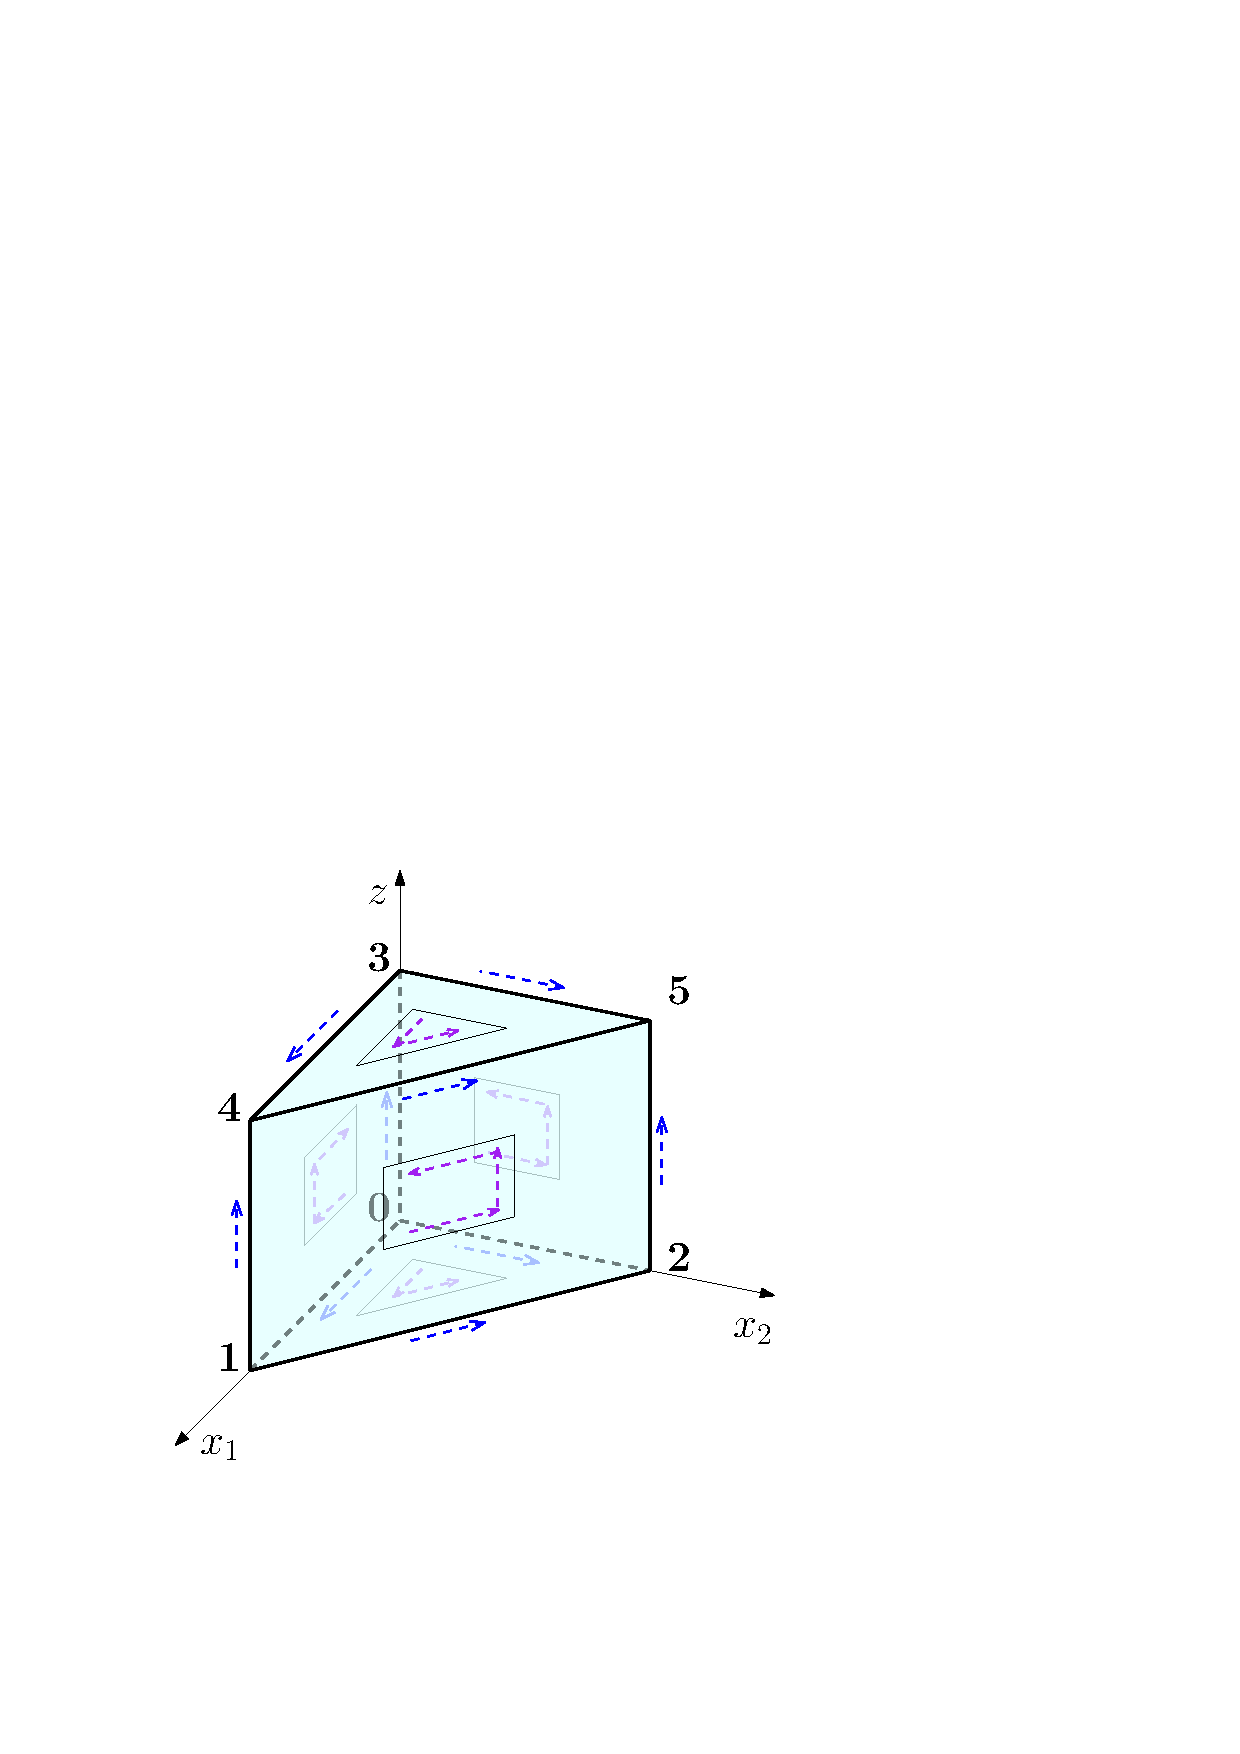
\includegraphics[scale=0.5]{./figures/MasterPrismOrientations.pdf}
\caption{Master prism with numbered vertices \textit{and} local edge and face orientations.}
\label{fig:MasterPrismOrientations}
\end{center}
\end{figure}

To construct orientation embedded shape functions for the prism, it is recommended to have read \S\ref{sec:HexaOrientations} and \S\ref{sec:TetOrientations}.
The predefined \textit{local} edge and face orientations for the prism are illustrated in Figure \ref{fig:MasterPrismOrientations}.
They represent the $\oo=0$ case.
The task at hand is to find the associated \textit{locally ordered} tuples of affine coordinates representing those local orientations.
As usual, the key is being aware of the relationships between the vertices and the affine coordinates.
As examples take edges 01 and 03, and faces 012 and 0143.
%As examples take mixed edge 01, quadrilateral edge 03, triangle face 012 and quadrilateral face 0143.

For mixed edge 01, the vertices are $v_0$ and $v_1$, which are linked to $(\nu_0(x),\mu_0(z))$ and $(\nu_1(x),\mu_0(z))$ respectively.
The only difference is that $v_0$ is linked to $\nu_0(x)$, while $v_1$ is linked to $\nu_1(x)$.
The local orientation for edge 01 is represented by the local vertex-ordering $v_0\tdashto v_1$.
Therefore, the locally ordered pair for edge 01 is $\vec{\nu}_{01}(x)=(\nu_0(x),\nu_1(x))$.
The orientation embedded shape functions for mixed edge 01 are simply the usual shape functions, but with their respective ancillary operator and differential form (that is $\phi_i^\E$, $E_i^\E$, $\nabla\phi_i^\E$ and $\nabla\times E_i^\E$) being precomposed with $\sigma_\oo^\E$ and evaluated at the locally ordered pair.

For quadrilalteral edge 03, composed of vertices $v_0$ and $v_3$, the differing affine coordinates are $\mu_0(z)$ and $\mu_1(z)$ respectively.
Since the local vertex-ordering is $v_0\tdashto v_3$, it follows the locally ordered pair for this edge is $\vec{\mu}_{01}(z)$.
Then, the orientation embedded shape functions are constructed like those of mixed edge 01.
That is, precomposing the ancillary operators with $\sigma_\oo^\E$ and evaluating at the locally ordered pair.

For triangle face 012, composed of vertices $v_0$, $v_1$ and $v_2$, the differing affine coordinates are $\nu_0(x)$, $\nu_1(x)$ and $\nu_2(x)$ respectively.
The local vertex-ordering is $v_0\tdashto v_1\tdashto v_2$, so the locally ordered triplet for this edge is $\vec{\nu}_{012}(x)$.
Then, the orientation embedded shape functions are the usual shape functions but with the ancillary operators ($\phi_{ij}^\Tri$, $E_{ij}^\Tri$, $V_{ij}^\Tri$, $\nabla\phi_{ij}^\Tri$, $\nabla\times E_{ij}^\Tri$ and $\nabla\cdot V_{ij}^\Tri$) precomposed with $\sigma_\oo^\Tri$ and evaluated at the locally oriented triplet.

Finally, quadrilateral face 0143 has local vertex-ordering $v_0\tdashto v_1\tdashto v_4\tdashto v_3$, so one only needs to look at $v_0\tdashto v_1$ and $v_1\tdashto v_4$ as if they were edges.
This leads to the locally ordered pairs $\vec{\nu}_{01}(x)$ and $\vec{\mu}_{01}(z)$ respectively, so the locally ordered quadruple is $(\vec{\nu}_{01}(x),\vec{\mu}_{01}(z))$.
Again, the orientation embedded shape functions are simply the shape functions but with the ancillary operators ($\phi_{ij}^\square$, $E_{ij}^\square$, $V_{ij}^\square$, $\nabla\phi_{ij}^\square$, $\nabla\times E_{ij}^\square$ and $\nabla\cdot V_{ij}^\square$) precomposed with $\sigma_\oo^\square$ and evaluated at the locally oriented quadruple.


%Some info maybe
%The orientations for the prism are dealt much the same way as with the hexahedron and tetrahedron, but in the prism there are two types of edges and two types of faces.
%The two types of edges are treated very similarly, as expected, while the faces are treated separately, since the concept of orientation differs for triangle and quadrilateral faces.
%In any case, the local axes or local numbering, which are fixed at the master element level, are important since they constitute the orientation $\oo=0$ basis case.
%These local axes and numbering are shown in Figure (\textit{add Figure}).%specified in Appendix \ref{app:Enumeration}.
%
%Note that any given vertex is associated to one triangle affine coordinate $\nu_a$ and one edge affine coordinate $\mu_c$, so that indeed its $H^1$ vertex function is precisely $\nu_a\mu_c$ (see \S\ref{sec:PrismH1vertices}).
%The vertices in the bottom triangle face (vertices 0, 1 and 2) are related to $\mu_0$ while those in the top face (vertices 3, 4 and 5) are related to $\mu_1$.
%At the same time, vertices $a$ and $a+3$ are associated to $\nu_a$, for $a=0,1,2$.
%These associations are convenient when explaining the orientations in the case of the prism. 
%
%\subsubsection{Edge Orientations}
%Edge functions, and hence edge orientations are only valid in $H^1$ and $H(\mathrm{curl})$. 
%The treatment is the same for both spaces, with the edge functions $\phi_i^\E$ and $E_i^\E$ being replaced by their oriented versions $\phi_i^{\e,\oo}$ and $E_i^{\e,\oo}$.
%Recall for edges there are only two possible orientations given by the orientation parameter $\oo=0,1$.
%They are explained in \S\ref{sec:edgeorientations}.
%Regardless of the type of edge, the first step is always to look at the local axis, which will determine the order in which the entries are specified in $\phi_i^{\e,\oo}$ and $E_i^{\e,\oo}$, and represents the $\oo=0$ case.
%For completeness, some examples are given below.
%
%\paragraph{Mixed Edges.} Take for example edge 34. 
%Here, vertex 3 is associated to the affine coordinate $\nu_0$, while vertex 4 is related to $\nu_1$. 
%Both are also related to $\mu_1$, since they lie in the top triangle. 
%The local edge axis for this edge points from vertex 3 ($\nu_0$) to vertex 4 ($\nu_1$), meaning that order of the entries in $\phi_i^{\e,\oo}$ and $E_i^{\e,\oo}$ for the mixed edge shape functions associated to this edge should be $(\nu_0(x),\nu_1(x))$. Hence, for instance, the $H^1$ mixed edge shape functions shown in \eqref{eq:PrismH1mixededges} would become
%\begin{equation*}
%	\phi_i^\mathrm{e}=\mu_1\phi_i^{\e,\oo}(\nu_0,\nu_1)
%  	=\begin{cases}
%    	\mu_1\phi_i^{\e,0}(\nu_0,\nu_1)=\mu_1\phi_i^{\e}(\nu_0,\nu_1)\,\,\,\text{if }\oo=0\\
%        \mu_1\phi_i^{\e,1}(\nu_0,\nu_1)=\mu_1\phi_i^{\e}(\nu_1,\nu_0)\,\,\,\text{if }\oo=1\,,
%        \end{cases}
%\end{equation*}
%where $i=2,\ldots,p$. Here, in $\phi_i^{\e,\oo}$, the orientation $\oo=1$ case is managed simply by permuting the indices, as described in \S\ref{sec:edgeorientations}. The same applies to the gradients of these $H^1$ functions and to the $H(\mathrm{curl})$ mixed edge functions and their curl, which involve $E_i^{\e,\oo}$ instead.
%
%\paragraph{Quadrilateral Edges.} Take for example edge 25. 
%Vertices 2 and 5 are related to affine coordinates $\mu_0$ and $\mu_1$ respectively, and both are also related to $\nu_2$.  
%The local axis points from vertex 2 ($\mu_0$) to vertex 5 ($\mu_1$), so that the entries in $\phi_i^{\e,\oo}$ and $E_i^{\e,\oo}$ should be $(\mu_0(z),\mu_1(z))$. 
%More explicitly, the $H^1$ quadrilateral edge shape functions shown in \eqref{eq:PrismH1quadedges} would then be
%\begin{equation*}
%	\phi_i^\mathrm{e}=\nu_2\phi_i^{\e,\oo}(\mu_0,\mu_1)
%  	=\begin{cases}
%    	\nu_2\phi_i^{\e,0}(\mu_0,\mu_1)=\nu_2\phi_i^{\e}(\mu_0,\mu_1)\,\,\,\text{if }\oo=0\\
%        \nu_2\phi_i^{\e,1}(\mu_0,\mu_1)=\nu_2\phi_i^{\e}(\mu_1,\mu_0)\,\,\,\text{if }\oo=1\,,
%        \end{cases}
%\end{equation*}
%where $i=2,\ldots,q$. Again, the same applies to the gradients of these functions and to the $H(\mathrm{curl})$ quadrilateral edge functions and their curl.
%
%\subsubsection{Face Orientations}
%\label{sec:PrismFaceOrientations}
%Face functions (and face orientations) exist in $H^1$, $H(\mathrm{curl})$ and $H(\mathrm{div})$.
%The treatment is analogous for all the spaces, with the triangle face functions $\phi_{ij}^\Tri$, $E_{ij}^\Tri$, $E_{ij}^\Tri}$, and $V_{ij}^\Tri$ and quadrilateral functions $\phi_{ij}^\square$, $E_{ij}^{\square_I}$, $E_{ij}^{\square_{II}}$, and $V_{ij}^\square$, being replaced by their oriented versions $\phi_{ij}^{\Tri,\oo}$, $E_{ij}^{\Tri_I,\oo}$, $E_{ij}^\Tri,\oo}$, $V_{ij}^{\Tri,\oo}$, $\phi_{ij}^{\square,\oo}$, $E_{ij}^{\square_I,\oo}$, $E_{ij}^{\square_{II},\oo}$, and $V_{ij}^{\square,\oo}$. 
%
%\paragraph{Triangle Faces.}
%Triangle face orientations are explained in \S\ref{sec:TriaFaceOrientations}. 
%Here, there are six possible orientations represented by the orientation parameter $\oo=0,\ldots,5$.
%As usual, the first step is to look at the local face numbering.
%For instance, take the top face 345. 
%The vertices 3, 4 and 5 are associated to the affine functions $\nu_0$, $\nu_1$ and $\nu_2$ respectively, and the three are also related to $\mu_1$.
%The local numbering for this face goes from vertex 3 ($\nu_0$) to vertex 4 ($\nu_1$) to vertex 5 ($\nu_2$), so that the order of the entries in  $\phi_{ij}^{\Tri,\oo}$, $E_{ij}^{\Tri_I,\oo}$, $E_{ij}^\Tri,\oo}$, and $V_{ij}^{\Tri,\oo}$ is simply $(\nu_0(x),\nu_1(x),\nu_2(x))$.
%For example, the $H^1$ triangle face shape functions in \eqref{eq:PrismH1TriFace} turn out to be
%\begin{equation*}
%		\phi_{ij}^\mathrm{f}=\mu_1\phi_{ij}^{\Tri,\oo}(\nu_0,\nu_1,\nu_2)=\begin{cases}
%    \mu_1\phi_{ij}^{\Tri}(\nu_0,\nu_1,\nu_2)&\quad\text{if  }\,\oo=0\\
%    \mu_1\phi_{ij}^{\Tri}(\nu_2,\nu_0,\nu_1)&\quad\text{if  }\,\oo=1\\
%    \mu_1\phi_{ij}^{\Tri}(\nu_1,\nu_2,\nu_0)&\quad\text{if  }\,\oo=2\\
%    \mu_1\phi_{ij}^{\Tri}(\nu_0,\nu_2,\nu_1)&\quad\text{if  }\,\oo=3\\
%    \mu_1\phi_{ij}^{\Tri}(\nu_1,\nu_0,\nu_2)&\quad\text{if  }\,\oo=4\\
%    \mu_1\phi_{ij}^{\Tri}(\nu_2,\nu_1,\nu_0)&\quad\text{if  }\,\oo=5\,,
%    \end{cases}
%\end{equation*}
%for $i\geq2$, $j\geq1$ and $n=i+j=3,\ldots,p$. 
%Here, the permutation of the entries depending on the orientation $\oo$ is determined by the auxiliary function $\vec{\sigma}$ which is discussed in \S\ref{sec:TriaFaceOrientations}. 
%Obviously the same arguments apply to the other triangle face functions in $H(\mathrm{curl})$ and $H(\mathrm{div})$ and their differential forms.
%
%\paragraph{Quadrilateral Faces.}
%Quadrilateral face orientations are discussed in \S\ref{sec:QuadFaceOrientations}.
%In this case there are eight possible orientations represented by the orientation parameter $\oo=0,\ldots,7$.
%Take for example face 1254.
%The local numbering goes from vertex 1 (related to $\nu_1$) to vertex 2 (related to $\nu_2$ and $\mu_0$) to vertex 3 (related to $\mu_1$) and to vertex 4.
%Here, the first two elements of the local numbering, vertex 1 with $\nu_1$ to vertex 2 with $\nu_2$, determine the \textit{first} coordinate pair, which is $(\nu_1(x),\nu_2(x))$.
%The second and third elements of the local numbering, vertex 2 with $\mu_0$ to vertex 3 with $\mu_1$, determine the \textit{second} coordinate pair, which is  $(\mu_0(z),\mu_1(z))$.
%These two coordinate pairs constitute the $\oo=0$ orientation, so they are precisely the entries of $\phi_{ij}^{\square,\oo}$, $E_{ij}^{\square_I,\oo}$, $E_{ij}^{\square_{II},\oo}$, and $V_{ij}^{\square,\oo}$. For instance, the $H^1$ quadrilateral shape functions in \eqref{eq:PrismH1QuadFace} become
%\begin{equation*}
%    \phi_{ij}^\mathrm{f}=\phi_{ij}^{\square,\oo}(\nu_1,\nu_2,\mu_0,\mu_1)=\begin{cases}
%    \phi_{ij}^\square(\nu_1,\nu_2,\mu_0,\mu_1)&\quad\text{if  }\,\oo=0\\
%    \phi_{ij}^\square(\mu_1,\mu_0,\nu_1,\nu_2)&\quad\text{if  }\,\oo=1\\
%    \phi_{ij}^\square(\nu_2,\nu_1,\mu_1,\mu_0)&\quad\text{if  }\,\oo=2\\
%    \phi_{ij}^\square(\mu_0,\mu_1,\nu_2,\nu_1)&\quad\text{if  }\,\oo=3\\
%    \phi_{ij}^\square(\mu_0,\mu_1,\nu_1,\nu_2)&\quad\text{if  }\,\oo=4\\
%    \phi_{ij}^\square(\nu_2,\nu_1,\mu_0,\mu_1)&\quad\text{if  }\,\oo=5\\
%    \phi_{ij}^\square(\mu_1,\mu_0,\nu_2,\nu_1)&\quad\text{if  }\,\oo=6\\
%    \phi_{ij}^\square(\nu_1,\nu_2,\mu_1,\mu_0)&\quad\text{if  }\,\oo=7\,,
%    \end{cases}
%\end{equation*}
%where the numbering is $i=2,\ldots,p$, $j=2,\ldots,q$ if $\oo=0,2,5,7$, and $i=2,\ldots,q$, $j=2,\ldots,p$ if $\oo=1,3,4,6$.
%The permutation of the entries is actually determined by the auxiliary function $\vec{\kappa}$ which is explained in \S\ref{sec:QuadFaceOrientations}.
%The same applies to $E_{ij}^{\square_I,\oo}$, $E_{ij}^{\square_{II},\oo}$, $V_{ij}^{\square,\oo}$ and their differential forms.

